\documentclass[titlepage,11pt]{article}
\usepackage[a4paper]{geometry}
\usepackage[centertags]{amsmath}            % higher mathematics (AMS)
\usepackage{amsfonts}                       % higher mathematics symbols (AMS)
\usepackage{graphicx}                       % graphics extensions
\usepackage{rotating}                       % rotate eps-figures
\usepackage{caption}                        % nicer figure-captions
\usepackage{exscale}                        % scale math-symbols correctly
\usepackage[german]{babel}                  % extensions for german
\usepackage[utf8]{inputenc}                 % enable UTF-8
\usepackage[T1]{fontenc}
\usepackage[babel=true]{csquotes}
\usepackage{epsfig,epic,eepic}              % Xfig- and EPS-figures
\usepackage{fancyhdr}                       % some fancy headings
\usepackage[backend=biber,style=authoryear,bibencoding=utf8]{biblatex}
\addbibresource{bibtex/diplom.bib}
\addbibresource{bibtex/chaos.bib}
\addbibresource{bibtex/neuro.bib}

% some hacks before we start
\pagestyle{fancyplain}
%
% change fonts fort section titles and captions
%
\makeatletter                                           % allow use of '@' sign
\renewcommand{\section}{\@startsection%                 %
{section}{1}{\z@}%                                      %
{-3.5ex \@plus -1ex \@minus -.2ex}%                     %
{2.3ex \@plus.2ex}%                                     %
{\reset@font\Large\bfseries\sffamily}}%                 %
\renewcommand{\subsection}{\@startsection%              %
{subsection}{2}{\z@}%                                   %
{-3.25ex\@plus -1ex \@minus -.2ex}%                     %
{1.5ex \@plus .2ex}%                                    %
{\reset@font\large\bfseries\sffamily}}                  %
\renewcommand{\subsubsection}{\@startsection%           %
{subsubsection}{3}{\z@}%                                %
{-3.25ex\@plus -1ex \@minus -.2ex}%                     % new font for \section etc.
{1.5ex \@plus .2ex}%                                    %
{\reset@font\normalsize\bfseries\sffamily}}	            %
\renewcommand{\paragraph}{\@startsection%               %
{paragraph}{4}{\z@}%                                    %
{3.25ex \@plus1ex \@minus.2ex}%                         %
{-1em}%                                                 %
{\reset@font\normalsize\bfseries\sffamily}}             %
\renewcommand{\subparagraph}{\@startsection%            %
{subparagraph}{5}{\parindent}%                          %
{3.25ex \@plus1ex \@minus .2ex}%                        %
{-1em}%                                                 %
{\reset@font\normalsize\sffamily}}                      %
\makeatother                                            % protect use of '@' sign
\renewcommand{\captionlabelfont}{\bfseries\sffamily}    % captionlabelfont...


%
% miscellaneous stuff
%
\addtolength{\headwidth}{0.6\marginparwidth}            % make headline wider
\addtolength{\headheight}{2.5pt}                        % make headline higher
%\setlength{\plainheadrulewidth}{0.4pt}                 % plain headrule
\setlength{\parskip}{0.0pt}                             % no skip at new paragraph
%\setlength{\parindent}{0.0pt}                          % no indent at new paragraph


%
% some fancy headings and footnotes...
%
\renewcommand{\thefootnote}{\fnsymbol{footnote}}
\renewcommand{\sectionmark}[1]{\markboth{\uppercase{#1}}{\uppercase{#1}}}
\renewcommand{\subsectionmark}[1]{\markright{\thesubsection\ \ #1}}
\lhead[\fancyplain{\bfseries\thepage}{\bfseries\thepage}]{\fancyplain{}{\slshape\rightmark}}
\rhead[\fancyplain{}{\slshape\leftmark}]{\fancyplain{\bfseries\thepage}{\bfseries\thepage}}
\cfoot[]{}

\sloppy

% reset counter in every Section
\numberwithin{equation}{section}
%\numberwithin{footnote}{section}
\numberwithin{figure}{section}

% main()
\begin{document}
    \begin{titlepage}
\Large
\sffamily
\vfill

\begin{center}
{\bfseries\huge Nichtlineare Dynamik kolumn"arer\\[0.6ex] Strukturen im visuellen Cortex}

\vfill

{--- Diplomarbeit ---\\ vorgelegt von}

\bigskip
\bigskip

\rmfamily
\textsc{Frank Hoffs"ummer}
\sffamily

\vfill

\begin{figure}[h]
\begin{center}
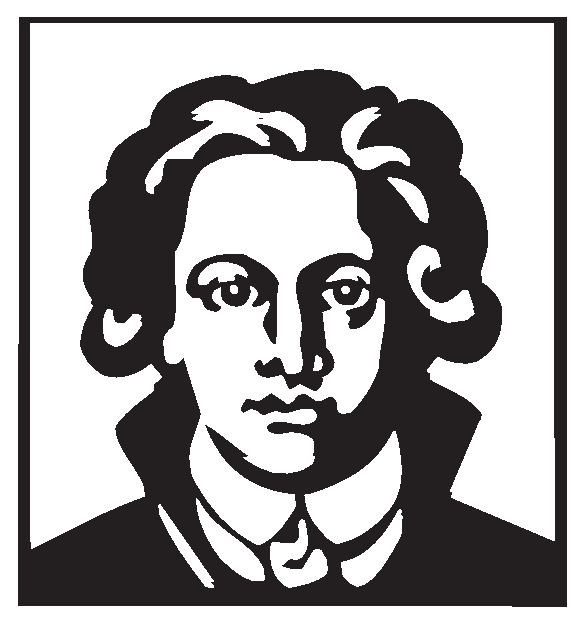
\epsfig{file=pics/goethe.eps,width=3cm}
\end{center}
\end{figure}

{Institut f"ur Theoretische Physik\\
Johann Wolfgang Goethe--Universit"at\\
Frankfurt am Main\\
Februar 1996}
\end{center}

\vfill
\normalsize
\normalfont
\end{titlepage}


\tableofcontents


    \section{Einleitung}
\label{einleitung}
\thispagestyle{plain}

\subsection{Physik im Hirn?}
%... stellt der darwinistischen evolution die sozio-kulturelle evolution zur
%seite, welche dieser teilweise entgegenwirkt.

Verglichen mit anderen Lebewesen auf diesem Planeten nimmt die Spezies
Mensch eine Ausnahmeposition ein.  Diese Sonderstellung wird nicht nur
durch morphologische Unterschiede zu unseren nächsten Verwandten wie
z.B. aufrechter Gang und umgestaltetes Gebiß gerechtfertigt. Sie fällt
dem Menschen vielmehr durch die besondere Ausprägung seines Gehirns,
insbesondere des Neocortex zu (siehe Abb.~\ref{hirnmasse}).  Das
menschliche Gehirn ist die komplexeste, uns bekannte Struktur im Universum.
Es besteht aus ca. $10^{12}$~Nervenzellen, von denen jede einzelne mit bis
zu tausenden anderen verbunden ist, und ist materielle und funktionale
Grundlage von Wahrnehmen, Empfinden, Erkennen, Lernen, Erinnern, Denken und
Mitteilen; auf seinen Prozessen beruht auch das Bewußtsein. Gleichwohl ist
das Gehirn sich selbst rätselhaft.

Seit ungefähr 100~Jahren gibt es ernstzunehmende Ansätze von
Naturwissenschaftlern, dieses Rätsel zu lösen.  Mittlerweile sind zu der
wissenschaftlichen Neugier klare wirtschaftliche und industrielle
Interessen hinzugekommen. So arbeiten in diesem Jahrzehnt --- vom Kongress
der Vereinigten Staaten zur ``Dekade des Hirns'' ausgerufen --- weltweit
Wissenschaftler aus allen Disziplinen daran, die Funktionsweise des
menschlichen Gehirns zu entschlüsseln. Von den Ergebnissen dieser
Forschungen erhofft man sich nicht nur ein besseres Verständnis
neurologischer Krankheitsbilder, wie z.B. der Parkinson'schen Krankheit und
der Multiplen Sklerose. (Dies könnte den Schlüssel zu deren Heilung,
zumindest jedoch Chancen auf bessere Therapien beinhalten.)

Eine besondere Motivation entspringt der Hoffnung, durch die Extraktion
einfacher Regeln und Funktionsprinzipien, die der Informationsverarbeitung
im menschlichen Gehirn zugrunde liegen, die Leistungsfähigkeit
künstlicher informationsverarbeitender Systeme bei bestimmten
Aufgabenstellungen (wie z.B. Mustererkennung, Sprachverständnis,
Spracherkennung, Bewegungskoordination) massiv zu steigern. Auch der sich
durch die ganze Kulturgeschichte ziehende Traum des Menschen von einem
eben--bürtigen, von Menschenhand geschaffenen Wesen, dem \emph{Humanoiden},
wäre dann in greifbare Nähe gerückt \parencite[zum Stand der Dinge siehe z.B.][]{brooks:1990}.

Auf dem Weg zu einem einheitlichen Verständnis von Hirnentwicklung und
\mbox{--funktion} können auch Physiker einen gewinnbringenden Beitrag leisten.
Die moderne Physik bietet eine Palette von Werkzeugen und Methoden zur
Analyse und Beschreibung komplexer Nicht--Gleichgewichts--Systeme.  Viele
der in der Theoretischen Physik an einfachen Systemen entwickelten Konzepte
können auf die Hirnforschung übertragen werden, und so auf einer
abstrakten Ebene zum qualitativen Verständnis beobachteter Phänomene
beitragen. Idealerweise werden dabei in der Theorie entwickelte Konzepte
und Modelle im Wechselspiel mit dem Experiment verfeinert. Oft lassen sich
aus solchen Modellen auch Vorhersagen und neue Fragestellungen ableiten.

Diese Ergänzung der experimentellen Hirnforschung um theoretische
Komponenten hat sich in der Vergangenheit bereits für beide Gebiete als
fruchtbar erwiesen: Durch Arbeiten von \textcite{hopfield:1982}
z.B. wurde die statistische Physik als geeigneter Rahmen für die Analyse
der Gedächtnisfunktion sowie der Verallgemeinerung beim Erlernen von
Regeln entdeckt.  Die Untersuchung pulsgekoppelter Neurone lieferte neue
Erkenntnisse über die nichtlinearen Synchronisationsmechanismen
oszillierender Systeme \parencite[siehe z.B.][]{ernst95a}.  In dieser
Arbeit werden Konzepte der Nichtlinearen Dynamik strukturbildender Systeme
verwendet, um Unterschiede in den visuellen Reizrepräsentationen im Hirn
von Katzen und Affen einheitlich zu erklären.  Langfristig dient die
Ausweitung des Kanons der Physik auf biologische Systeme wie z.B. dem
Gehirn wohl dem Erkenntnisfortschritt in beiden Gebieten, der Physik und
der Biologie \parencite{braitenberg:1977}.

\begin{figure}[t]
\centering
\epsfig{file=pics/hirngewicht.eps,width=9cm}
\caption{Man kann die Überentwicklung des menschlichen Hirns bereits
deutlich am Verhältnis zwischen Gehirn-- und Körpergewicht ablesen. Hier
dargestellt ist dieses Verhältnis in doppeltlogarithmischer Darstellung
für 476 Säugetierarten und den Menschen
\parencite[aus][]{martin:1995}. Das prozentuale Verhältnis ergäbe
eine Abweichung zugunsten leichtgewichtigerer Arten.  Der Wert für den
Menschen liegt am weitesten oberhalb der Allometriegeraden; unsere Spezies
hat also relativ zum Körpergewicht ``am meisten'' Hirn.}
\label{hirnmasse}
\end{figure}

\subsection{Überblick}

In der vorliegenden Arbeit wird ein Modell zur Beschreibung der
aktivitätsabhängigen, koordinierten Entwicklung neuronaler
Reizrepräsentationen (auch: neuronale Karten) untersucht.  Basierend auf
diesem Modell wird ein Szenarium vorgeschlagen, das die speziesabhängige
Erscheinung der Reizrepräsentationen aus dem primären visuellen Cortex
von Katzen und Affen einheitlich erklären kann.  Die Arbeit gliedert sich
wie folgt:

\begin{itemize}
\item Eine Einführung in die wichtigsten biologischen Grundbegriffe sowie
einen Über\-blick über die biologischen Phänomene, die in dieser Arbeit
behandelt werden, liefert Kapitel~\ref{biologie}. Hier werden auch
Ergebnisse einer Analyse experimenteller Daten vorgestellt, welche die
Wechselwirkung verschiedener neuronaler Karten untereinander aufzeigt.

\item In Kapitel~\ref{modell} wird das im folgende verwendete,
phänomenologische Modell zur Simulation der koordinierten Entwicklung
visueller neuronaler Karten vorgestellt. Wichtige Eigenschaften des Modells
erschließen sich durch eine lineare Stabilitätsanalyse: So zeigt sich,
daß die Strukturbildung des Modells kritisch von der
Kooperationsreichweite $\sigma$ abhängt.  Die Wellenlängen der
entstehenden Strukturen lassen sich durch geeignete Parameterwahl
vorbestimmen, und können so an biologische Vorbilder angepasst werden.
Darüber hinaus gibt die lineare Stabilitätsanalyse Auskunft über die
Zeitskala der strukturbildenden Dynamik.

\item In Kapitel~\ref{main} wird dann ein Szenarium entwickelt, mit dessen
Hilfe sich die in Kapitel~\ref{biologie} skizzierten Speziesunterschiede
visueller Reizrepräsentationen einheitlich erklären lassen.  Die
numerischen Untersuchungen dieses Szenariums anhand des in
Kapitel~\ref{modell} eingeführten Modells ergeben Karten, die sehr gut mit
den beobachteten Karten aus Affen und Katzen übereinstimmen.

\item Die Arbeit schließt mit einer Diskussion der Ergebnisse in Kapitel
~\ref{zusammenfassung}. Unter Voraussetzung der Allgemeingültigkeit des
Szenariums werden Vorhersagen über die Entstehungsreihenfolge neuronaler
Karten in anderen Spezies gemacht. Alternative Erklärungsansätze werden
diskutiert und Experimente zur Verifikation des Szenariums vorgeschlagen.
\end{itemize}

    \section{Biologische Grundlagen}
\label{biologie}
\thispagestyle{plain}

Das visuelle System gehört zu den am gründlichsten untersuchten
Sinnessystemen der Großhirnrinde.  Das liegt nur zum einen an der gut
zugänglichen Lage der Cortexareale, die für die erste visuelle
Reizverarbeitung zuständig sind.  Sie befinden sich bei Säugern direkt
unterhalb der Schädeldecke im hinteren Pol des Großhirns.  Zum anderen
kann man das visuelle System einfach und unter kontrollierten,
reproduzierbaren Bedingungen über die Augen reizen. Es ist sozusagen das
``Wasserstoff--Atom der Hirnforschung''; theoretische Konzepte und
Erklärungsmodelle lassen sich im Experiment am visuellen System
falsifizieren, bzw. können im Wechselspiel mit dem Experiment verfeinert
werden.

In den folgenden Abschnitten werden die für das weitere Verständnis der
Arbeit benötigten biologischen Zusammenhänge, sowie die in dieser Arbeit
behandelten Phänomene erläutert. Der letzte Abschnitt dieses Kapitels
geht dabei auf Ergebnisse einer Datenanalyse ein, bei der in Zusammenarbeit
mit Siegrid Löwel vom Max--Planck--Institut für Hirnforschung die
geometrische Beziehung zwischen Okulardominanz-- und Orientierungskarten
aus A17 schielender Katzen untersucht wurde.

\subsection{Skizze des visuellen Systems von Säugern}

\subsubsection{Die Sehbahn}
\label{sehbahnkap}

Die Netzhaut (Retina) ist eine, aus drei verschiedenen Zelltypen
bestehende, schichtartig aufgebaute Struktur, welche die Umwandlung
physikalischer Lichtreize in neuronale Signale vornimmt.  Der schichtartige
Aufbau ist dabei charakteristisch für viele andere Strukturen im
Zentralnervensystem. Durch einfallendes Licht wird zunächst eine beim
Menschen aus ca. 125~Millionen Photorezeptoren (Stäbchen und Zapfen)
bestehende Zellschicht stimuliert.  Die visuelle Information wird dann in
einer zwischengelagerten Zellschicht und in einer Schicht aus
ca. 1~Millionen Ganglienzellen weiterverarbeitet. Die Nervenendungen
(Axone) der Ganglienzellen bündeln sich an der Papille und verlassen das
Auge als Sehnerv. Schon aus diesem anatomischen Verhältnis von 125:1 wird
deutlich, daß in der Retina eine Vorverarbeitung visueller Information
stattfinden muß (vgl. Abschn.~\ref{rf}).  Die Sehnerven aus beiden Augen
verzweigen sich im \emph{Chiasma opticum}: hier wechselt etwa die Hälfte
aller Sehnervfasern die Hemisphäre, während der Rest ungekreuzt
weiterverläuft (siehe Abb.~\ref{sehbahn}).  Alle Nervenfasern, die aus den
jeweils linken Netzhauthälften entstammen, werden so in die linke
Hirnhälfte weitergeleitet (analog bei der rechten Netzhauthälfte).  Auf
diese Weise ist hinter dem Chiasma opticum die rechte Gesichtsfeldhälfte
in der linken Hemisphäre und die linke in der rechten Hemisphäre
repräsentiert.  Nur ein kleiner Bereich des zentralen Gesichtsfeldes ist
beidseitig vertreten.

In jeder Hemisphäre projiziert nun ein Teil des neuzusammengesetzten
Nervenfaserbündels (\emph{Tractus opticus}) auf den seitlichen Kniehöcker
(\emph{Corpus geniculatum laterale}, LGN) im Thalamus.  Die gebündelten
Fasern aus den Netzhäuten werden hier in geordneter Weise wieder
aufgefächert und münden in mehreren Zellschichten, die wie in einem
Sandwich übereinander liegen.  Einzelne Kniehöckerzellen erhalten nur
Eingänge von einem Auge: Eine Zelle im LGN ist entweder ``linksäugig''
oder ``rechtsäugig''.  Diese beiden Zellsorten liegen getrennt voneinander
in verschiedenen Schichten.

\begin{figure}[t]
\centering
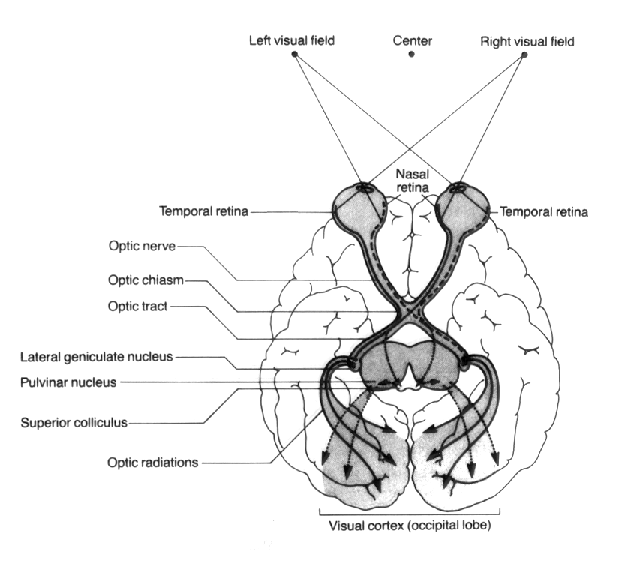
\epsfig{file=pics/sehbahn.eps,width=12cm}
\caption{Skizze der Sehbahn im menschlichen Gehirn von den Augen bis zum
primären visuellen Cortex \protect\citeaffixed{churchland:1992}{aus}.}
\label{sehbahn}
\end{figure}

Am Ende des LGN treten Nervenfasern aus allen Schichten zu einem breiten
Band zusammen, der \emph{Radiatio optica}, das zur Sehrinde aufsteigt.  Die
Sehrinde ist in mehrere abgegrenzete Gebiete, sogenannte \emph{Areale}
unterteilt, die zum Teil sehr spezifische Leistungen (wie z.B.
Bewegungs--, Form-- und Farbsehen) erbringen und in zahlreichen Kanälen
untereinander Information austauschen.  Das außenweltnächste,
\emph{primäre} visuelle Areal (in Affen V1, in Katzen häufig A17 genannt)
ist --- wie die Retina und das LGN --- schichtartig strukturiert.  Im Affen
projiziert das LGN ausschließlich zum primären visuellen Cortex, in
Katzen auch in umliegende Areale.  Auch bei der Projektion vom LGN in den
primären visuellen Cortex fächern die Fasern wieder in geordneter Weise
auf: Die Topologie der Abbildung vom Gesichtsfeld in den Cortex bleibt
somit erhalten.

\begin{figure}[t]
\centering
\begin{minipage}[m]{5cm}
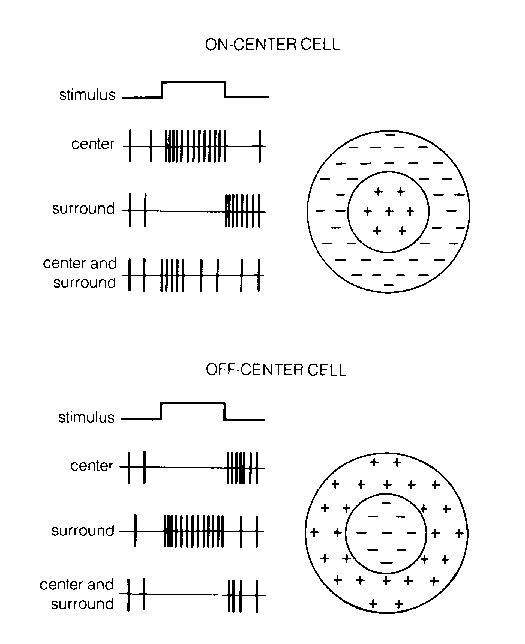
\epsfig{file=pics/rf_onoff.eps,width=5cm}
\end{minipage}
\hskip1cm
\begin{minipage}[m]{6cm}

\epsfig{file=pics/rf_simple.eps,width=6cm}
\end{minipage}
\caption{\textbf{a)} Skizze der radialsymmetrischen rezeptiven Felder
sogenannter ``Zentrum--Umfeld--Zellen'' (rechts). Die mit~``$+$''
markierten Gebiete kennzeichnen Bereiche, in denen eine Stimulation zur
Erregung der Zelle führt (``Exzitation''); in den mit~``$-$'' markierten
Bereichen führt eine Stimulation zur Hemmung der Zelle
(``Inhibition''). Nach ihrem Antwortverhalten (skizziert in der linken
Spalte) unterscheidet man 2 Typen: \emph{ON--Zentrum}--Zellen und
\emph{OFF--Zentrum}--Zellen. \textbf{b)} Skizze eines rezeptiven Feldes
einer sog. ``einfachen Zelle''. Ein zentrales, schmales exzitatorisches
Gebiet ist von symmetrischen, inhibitorischen Gebieten umgeben. Der
optimale Stimulus für diese Zelle ist ein vertikal orientierter
Lichtbalken (von $\approx1^\circ\times 8^\circ$ Größe) im Zentrum des
rezeptiven Feldes.}
\label{rfsimple}
\end{figure}

\subsubsection{Rezeptive Felder}
\label{rf}

Bei den Zellen im primären visuellen Cortex stellt man --- wie auch bei
den Ganglienzellen der Retina und den Zellen im LGN --- eine
Spezialisierung auf gewisse Reizmerkmale fest.  Dabei bestimmen in der
Retina zunächst wenige einfache Merkmale, wie z.B.  Position und Größe
eines Reizes, das Antwortverhalten einer Ganglienzelle (jede Zelle im
Zentralnervensystem hat eine Ruheaktivität, die bei geeigneter Stimulation
drastisch erhöht werden kann).  Das Gebiet genau abgegrenzter Position und
Größe auf der Sinnesoberfläche, welches bei Stimulation zur Aktivierung
einer Zelle führt --- also der Verantwortungsbereich dieser Zelle ---
bezeichnet man auch als das \emph{rezeptive Feld} dieser Zelle (siehe
Abb.~\ref{rfsimple}a).  Am Ende der Sehbahn reagieren die Zellen auf immer
abstraktere Merkmale der Außenwelt.  So lassen sich die Zellen im
primären visuellen Cortex oft nur noch mit Lichtreizen einer ganz
bestimmten Position, Größe und Orientierung stimulieren (einfache Zellen,
siehe Abb.~\ref{rfsimple}b).  Eine andere Zellsubpopulation erhöht ihre
Aktivität nur, wenn sich der Stimulus in einer bestimmten Richtung bewegt
(komplexe Zellen).  Zusätzlich sind die Zellen hier spezialisiert auf
Stimuli aus einem bestimmten Auge (man nennt dies ``okulare Dominanz'' der
Zellen).

Etwas verallgemeinernd bezeichnet man oft auch die Menge aller Merkmale,
die ein Reiz besitzen muß, um die Aktivität einer bestimmten Zelle zu
maximieren, als das rezeptive Feld dieser Zelle.  Die Zunahme der
Spezialisierung ist Ausdruck der Konvergenz im visuellen System: entlang
der Sehban erhalten fast alle Zellen Eingänge von mehr als einer anderen,
vorgelagerten Zelle. (Mit dieser anatomischen Beobachtung läßt sich
bereits die Präferenz visueller corticaler Zellen für bestimmte
Stimulusorientierungen erklären; siehe Abb.~\ref{opmodel}.)

\begin{figure}[p]
\centering
\epsfig{file=pics/opmodel.eps,width=9cm}
\caption{Einfaches Model der Orientierungspräferenz \protect\cite{hubel:1962}:
Die Axone mehrerer Zentrum--Umfeld--Zellen konvergieren auf eine einfache
Zelle. Dadurch, daß die rezeptiven Felder der Zentrum--Umfeld--Zellen auf
der Sinnesoberfläche entlang einer Linie angeordnet sind, antwortet die
einfache Zelle selektiv auf Lichtbalken einer bestimmten Orientierung.}
\label{opmodel}

\begin{center}
\begin{minipage}[m]{5.5cm}
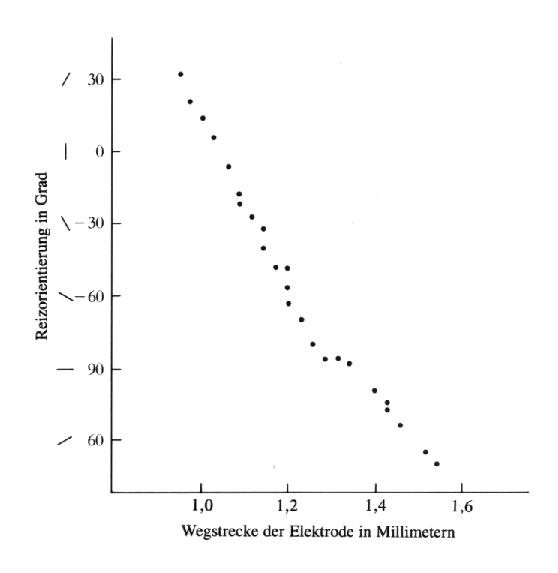
\epsfig{file=pics/opelektrode1.eps,width=5.5cm}
\end{minipage}
\hskip1cm
\begin{minipage}[m]{5.5cm}
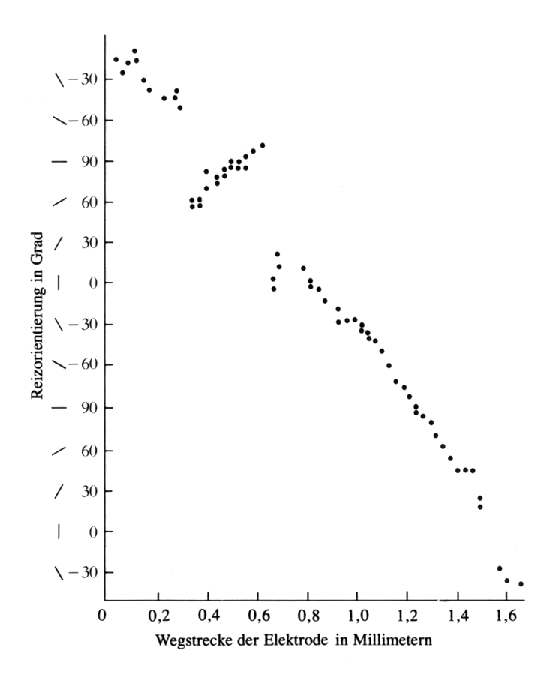
\epsfig{file=pics/opelektrode2.eps,width=5.5cm}
\end{minipage}
\end{center}
\caption{Ergebnis eines typischen Experiments mit tangentialer
Elektroden\-führ\-ung durch Area 17 in einer Katze für 2 verschiedene
Wegführungen, \protect\citeaffixed{hubel:1989}{aus}.  Aufgetragen ist
jeweils die präferierte Reizorientierung der abgeleiteten Zelle gegenüber
der Entfernung vom Ausgangspunkt der Messung.  \textbf{a)} Die bevorzugte
Reizorientierung ändert sich stetig und linear mit der Wegstrecke.
\textbf{b)} In dieser Messung ändert sich der Drehsinn zweimal sprunghaft
innerhalb einer Strecke von wenigen zehntel Millimetern.}
\label{opelektrode}
\end{figure}

\subsubsection{Kolumnäre Organisation der primären Sehrinde}

Mit einer Mikroelektrode, die schrittweise durch den Cortex geschoben wird,
kann man experimentell den Verlauf der rezeptiven Feldeigenschaften von
Zellen entlang einer Linie im Cortex bestimmen
\citeaffixed{hubel:1989}{siehe z.B.}: Durch die  Mikroelektrode ist
das elektrische Potential einer einzelnen Zelle meßbar.  Das
Aktionspotential einer Zelle im ``Ruhezustand'', also ohne geeignete
Stimulation, überschreitet dabei nur gelegentlich eine kritische Schwelle,
oberhalb der die Zelle einen elektrischen Puls aussendet (die Zelle
``feuert'').  Wird nun ein geeigneter Stimulus auf die Retina projiziert,
so können die Merkmale dieses Stimulus (wie z.B. Größe, Position, usw.)
solange variiert werden, bis die ``Feuerrate'' der betrachteten Zelle
maximiert wurde: das rezeptive Feld der Zelle wurde gefunden.  Auf diese
Weise können innerhalb eines Experiments die rezeptiven Felder mehrerer
Zellen bestimmt werden.

Ein Ergebnis solcher Messungen ist, daß die rezeptiven Feldeigenschaften
untereinanderliegender Zellen identisch sind. Tangential zur
Cortexoberfläche variieren die rezeptiven Feldeigenschaften der Zellen
dagegen i.a. graduell und in gesetzmäßiger Weise mit der Position der
Zellen auf der Cortexoberfläche (vgl. Abb.~\ref{opelektrode}).  Das
primäre visuelle Areal ist somit wie die meisten anderen
sinnesverarbeitenden Bereiche der Hirnrinde \emph{kolumnär} organisiert,
d.h.  Zellen sind zu funktionalen Einheiten (``Kolumnen'') von wenigen
Zehntelmillimetern Durchmesser zusammengefaßt, die sich zylinderförmig
radial in den Cortex erstrecken.

\subsection{Neuronale Karten}

Obwohl die Verschaltung der Retina mit dem primären visuellen Areal, wie
in Abschnitt~\ref{sehbahnkap} dargestellt, über mehrere
``Relaisstationen'' verläuft, bleibt die Topologie der Sinnesoberfläche
unter der Abbildung in den Cortex erhalten, d.h.  benachbarte Neurone im
Cortex haben benachbarte Verantwortungsbereiche im Gesichtsfeld.  Die im
letzten Abschnitt beschriebenen Mikroelektroden--Experimente ließen schon
früh erkennen, daß es sich bei dieser Projektion um eine
zweidimensionale, oftmals stetige Merkmalsabbildung handelt.  Aufgrund der
Nachbarschaftserhaltung läßt sich eine solche Abbildung auch als
\emph{Karte} der Außenwelt ansehen.  Unter einer \emph{neuronalen Karte}
versteht man eine (häufig in Ortskoordinaten) parametrisierte Darstellung
des Verlaufs einer rezeptiven Feldeigenschaft über ein Cortexareal.  Das
naheliegendste Beispiel einer neuronalen Karte ist die sogenannte
\emph{retinotope Karte} im primären visuellen Areal, bei der benachbarte
Neurone auf Reize reagieren, die benachbart im Gesichtsfeld angeordnet sind
(und deshalb benachbart auf die Retina abgebildet werden; dies erklärt das
Attribut ``retinotop'').

Im primären visuellen Cortex sind i.a. auch Karten abstrakterer Merkmale der
\mbox{Außenwelt} angelegt. Diese sind der retinotopen Karte überlagert.
Ein genaueres Bild dieser Karten für ein ausgedehntes Gebiet mit Hilfe von
Mikroelektroden--Experimenten zu erhalten hieße jedoch ``eine
dreidimensionale Frage mit einer eindimensionalen Meßmethode'' zu
beantworten \cite{hubel:1989}.  Mittlerweile gibt es jedoch geeignete
Methoden zur Messung neuronaler Karten. In den folgenden beiden Abschnitten
werden daher die wichtigsten Typen visueller neuronaler Karten zusammen mit
gebräuchlichen Methoden zu ihrer Messung vorgestellt.

\subsubsection{Okulardominanzkarten}
\label{odkarten}

\begin{figure}[t]
\centering
\begin{minipage}[m]{3.9cm}
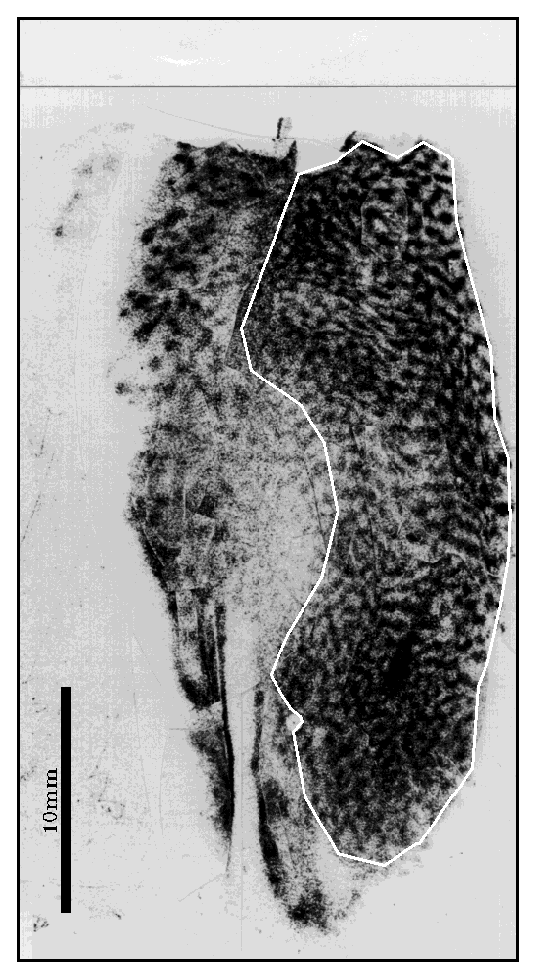
\epsfig{file=pics/normKatze.eps,width=3.9cm,clip=}
\end{minipage}
\hskip2cm
\begin{minipage}[m]{3.9cm}
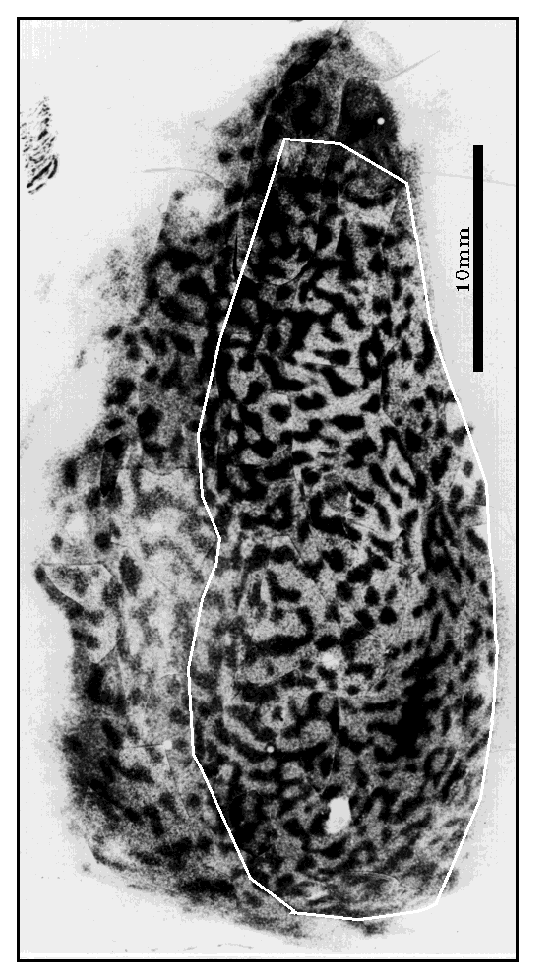
\epsfig{file=pics/strabKatze.eps,width=3.9cm}
\end{minipage}
\caption{Autoradiographie der Okulardominanzkarte aus A17 einer
normalsichtigen (links) und schielenden Katze (rechts)
\protect\citeaffixed{loewel:1987}{neurophysiologische Methode, Karten aus}.}
\label{odsiegrid}
\end{figure}

Neuroanatomische Verfahren zur Visualisierung einer
\emph{Okulardominanzkarte} beruhen auf radioaktiv markierten Stoffen
(typischerweise [$^3$H]--Prolin), die nach Injektion in ein Auge über
axonalen Transport von der Retina in den primären visuellen Cortex
gelangen.  Auf diese Weise reichert sich der radioaktive Marker in den
Zellen an, die in Verbindung mit dem markierten Auge stehen.

Physiologische Messungen solcher Karten verwenden radioaktiv markierte
2--deoxy\-glucose (2DG), die dem Versuchstier intravenös injiziert
wird. Danach wird ein Auge abgedeckt; der radioaktiv markierte Zucker
reichert sich nun in den Zellen an, die vom geöffneten Auge getrieben
werden. Auf diese Art und Weise läßt sich die funktionale Struktur der
Okulardominanz sichtbar machen.

\setcounter{footnote}{1}
In beiden Experimenten werden anschließend dünne Schnitte des Hirngewebes
angefertigt, die auf Glasplatten ausgefaltet und dann auf einen Film gelegt
werden. Nach langer Belichtung läßt sich anhand einer solchen
\emph{Autoradiographie} die Okularitätskarte als Schwärzungsverteilung
auf dem Film ablesen (siehe Abb.~\ref{odsiegrid}). Man erkennt eine
periodische Struktur, d.h. die schwarzen und weißen Gebiete (also die
Verantwortungsbereiche für markiertes/unmarkiertes bzw. aktives/inaktives
Auge) wechseln sich in bestimmten, regelmäßigen Abständen ab.
Untersuchungen der Wellenlänge\footnote{d.h. der über alle Richtungen
gemittelte Abstand, innerhalb dessen sich die Okulardominanz von einem Auge
zum anderen und wieder zurück verändert} von Okulardominanzkarten aus A17
normalsichtiger Katzen und A17 von Katzen, bei denen früh ein
künstlicher, divergenter Schielwinkel der Augen induziert wurde
(\emph{Strabismus}), zeigen daß die Wellenlänge der
Okulardominanzstruktur bei schielenden Katzen gegenüber der von
normalsichtigen Katzen systematisch erhöht ist \cite{loewel:1994}.
\setcounter{footnote}{1}

\subsubsection{Orientierungskarten}

Zur Messung von \emph{Orientierungskarten} benutzt man heute die
sogenannten \emph{optical imaging}--Verfahren, die Mitte der achtziger
Jahre entwickelt wurden. Diese Verfahren nutzen die veränderten optischen
Eigenschaften aktiver Zellen und ermöglichen dadurch die Sichtbarmachung
der funktionalen Anordung von Zellen unterhalb der Schädeldecke. Die
Veränderungen der optischen Eigenschaften können mit hochempfindlichen
Kameras durch die an einer Stelle geöffnete Schädeldecke des
Versuchstiers abfotographiert werden.  Auf diese Weise erhält man Karten
für beliebige, feste Stimulusmerkmale über ein ausgedehntes Gebiet von
einigen Millimetern Seitenlänge.

Eine der Methoden bedient sich spannungsempfindlicher Farbstoffe, die auf
die Oberfläche des primären visuellen Cortex aufgebracht werden. Das
Versuchstier sieht während des Experiments auf einen Bildschirm, auf dem
z.B. horizontal orientierte Balken durchlaufen. Die Zellen, die am
deutlichsten auf diese Stimulation antworten, äußern dies durch ihre
erhöhte elektrische Aktivität, welche wiederum die optischen
Eigenschaften des Farbstoffes verändert \cite{blasdel:1986,blasdel:1992a}.

Eine bessere Variante dieses Verfahrens ist durch Ausnutzung der
intrinsischen Signale der Cortexschicht nicht auf die langfristig
neurotoxischen, spannungsempfindlichen Farbstoffe angewiesen: Eine erhöhte
Aktivität der Zellen zieht einen erhöhten Blutdurchsatz in ihrer Umgebung
nach sich. Dieser erhöhte Blutdurchsatz äußert sich wiederum in einer
erhöhten Konzentration des Blutfarbstoffes Hämoglobin, der Licht der
Wellenlänge $800nm$ absorbiert. Mit CCD--Kameras kann man die
Intensitätsschwankungen auf der mit $800nm$--Licht beleuchteten
Cortexoberfläche aufnehmen. Die resultierende Hell/Dunkel--Verteilung
spiegelt die Inaktiv/Aktiv--Verteilung im beobachteten Gebiet wieder ---
also die neuronale Karte bezüglich des außen anliegenden Stimulus
\cite{lieke:1989,grinvald:1991}.

Orientierungskarten für eine feste Stimulusorientierung können auch mit
den in Abschnitt~\ref{odkarten} beschriebenen, neurophysiologischen
Methoden erhalten werden.  Der Vorteil des optischen Ableitens im Vergleich
zu neuroanatomischen oder neurophysiologischen Methoden liegt darin, daß
man in solchen Experimenten die neuronalen Karten \emph{in vivo}
erhält. Insbesondere ist man so in der Lage, während eines Experimentes
mehrere Karten für verschiedene Stimulusbedingungen von einem Versuchstier
abzuleiten.

\begin{figure}[t]
\centering
\begin{minipage}{10cm}
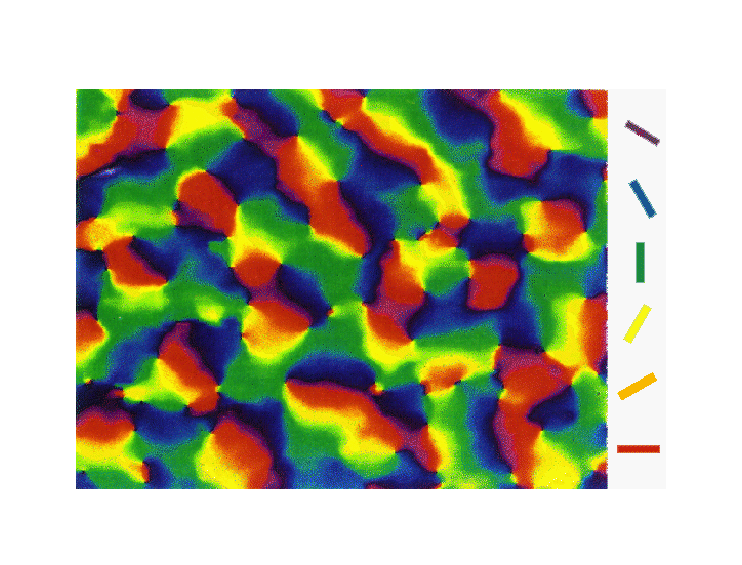
\epsfig{file=pics/OP_affe.eps,width=10cm}
\end{minipage}
\vskip0.5cm
\begin{minipage}[b]{4cm}
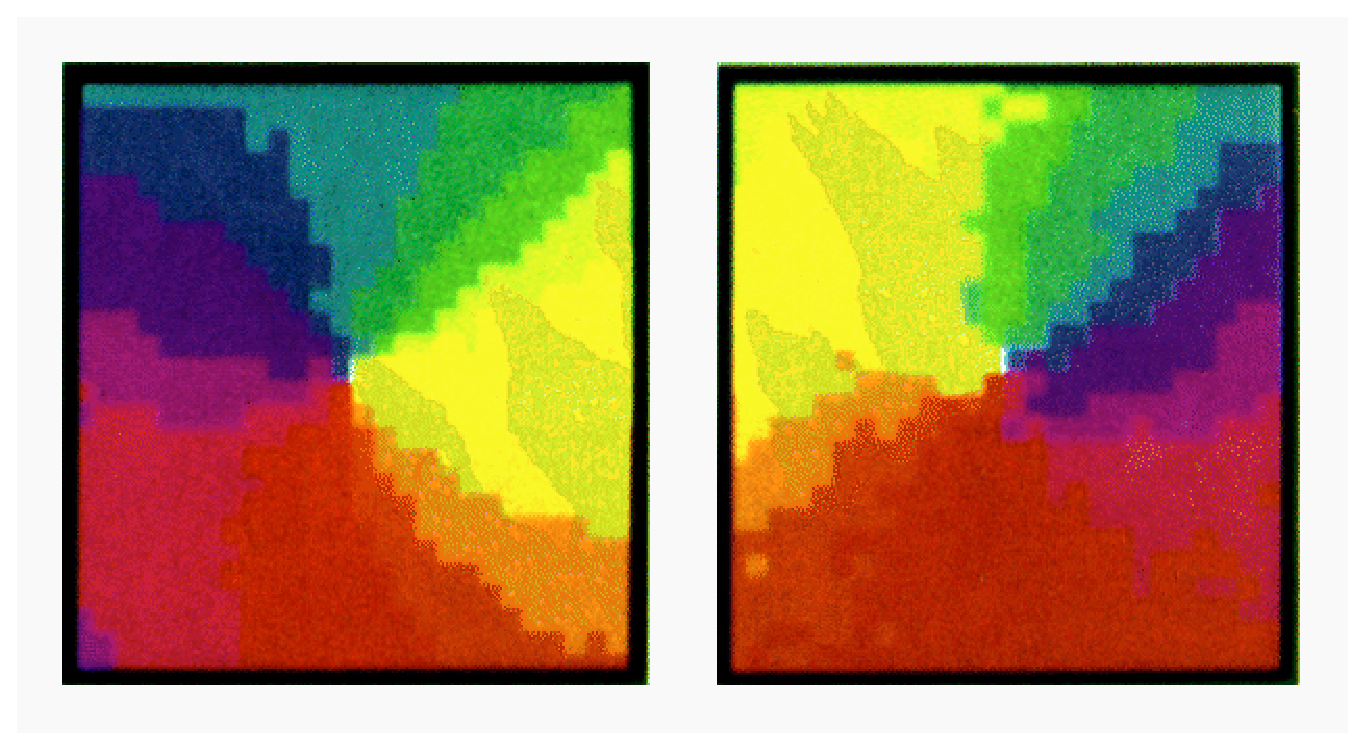
\epsfig{file=pics/pinwheels.eps,width=4cm}
\end{minipage}
\caption{\textbf{Oben:} Karte der Orientierungspräferenz aus dem primären
visuellen Cortex eines Makaken \protect\citeaffixed{blasdel:1992b}{aus}.
\textbf{Unten:} Beispiel für Pinwheels mit Chiralität~\eqref{chi}
$q_i=+\frac{1}{2}$ (links) und $q_i=-\frac{1}{2}$ (rechts). Die
Orientierung ändert sich beim linken Pinwheel im Uhrzeigersinn von gelb
nach rot (d.h. von rechts oblique nach horizontal); beim rechten Pinwheel
verläuft die Orientierungsänderung im Urzeigersinn von rot nach gelb
\protect\citeaffixed{bonhoeffer:1991}{d.h. von horizontal nach rechts
oblique; aus}.}
\label{opblasdel}
\end{figure}

Mehrere, in einem Versuch auf diese Art und Weise gemessenen
Aktivitäts\-ver\-tei\-lungen (auch ``single--condition'' Karten genannt, siehe
z.B. Abb.~\ref{layout}, rechte Spalte) für jeweils verschiedene
Orientierungen aus dem Intervall $[0^\circ,180^\circ)$ können dann
farblich codiert zu einer Orientierungskarte überlagert werden (siehe
Abb.~\ref{opblasdel}, oben).  Die Orientierungspräferenz als Funktion der
tangentialen Position $\mathbf{x}$ läßt sich folgendermaßen formulieren:

\begin{equation*}
z(\mathbf{x})=\sum\limits_k A_k(\mathbf{x})\; \text{e}^{i2\theta_k}
\label{zfeld}
\end{equation*}

Alle zu den Stimulusorientierungen $\theta_k$ gehörenden
Aktivitätsverteilungen $A_k(\mathbf{x})$ werden hier zu einem komplexen
Feld~$z$ überlagert.  Aus diesem Feld ergibt sich die Orientierungskarte
durch die Relation

\begin{equation*}
\vartheta=\frac{1}{2}\text{arctan}(z).
\end{equation*}

Das auffälligste Srukturelement einer solchen Orientierungskarte sind die
topologischen Punkt--Defekte, in deren Umgebung die
Iso--Orientierungsbereiche wie bei einem Windrad angeordnet sind (sie
werden daher oft auch als \emph{Pinwheels} berzeichnet): In einer
kreisförmigen Umgebung $C_i$ um eine Singularität ändert sich die
Orientierungspräferenz um $\pm 180^\circ$.  Die Positionen $\mathbf{x}_j$
dieser Singularitäten sind dabei die Nullstellen des komplexen Feldes
$z(\mathbf{x})$. Man unterscheidet zwei Sorten solcher Punkt--Defekte nach
ihrer ``Händigkeit'' (vgl. Abb.~\ref{opblasdel}, unten)

\begin{equation}
q_i=\frac{1}{2\pi}\oint_{C_i}\!\!\nabla\vartheta(\mathbf{x})\;ds = \pm
\frac{1}{2}
\label{chi}
\end{equation}

Beide Arten von Singularitäten treten gleich häufig auf.  In allen
natürlichen Karten ändert sich die Orientierungspräferenz bei einem
vollem Umlauf um eine solche Singularität immer nur um $\pm 180^\circ$,
nicht aber um $\pm 360^\circ$ \citeaffixed{penrose:1979}{einen Überblick
über alle theoretisch möglichen Arten solcher Punktdefekte gibt}.

Das nächst charakteristische Element einer Orientierungskarte sind die
sogenannten linearen Zonen. In diesen Gebieten, die etwa 50\% einer
Orientierungskarte ausmachen, laufen die Iso--Orientierungsbereiche
parallel über Strecken von bis zu $1mm$. Die Orientierung zwischen
benachbarten Iso--Orientierungsbereichen verändert sich stetig, d.h. ohne
Sprünge (das Ergebnis eines Mikrolektrodenexperiments, bei dem die
Mikroelektrode senkrecht zur Richtung einer solchen linearen Zone bewegt
wurde, zeigt Abb.~\ref{opelektrode}a).

\subsection{Speziesunterschiede visueller Reizrepräsentationen}
\label{unterschiede}

\begin{figure}[p]
\centering
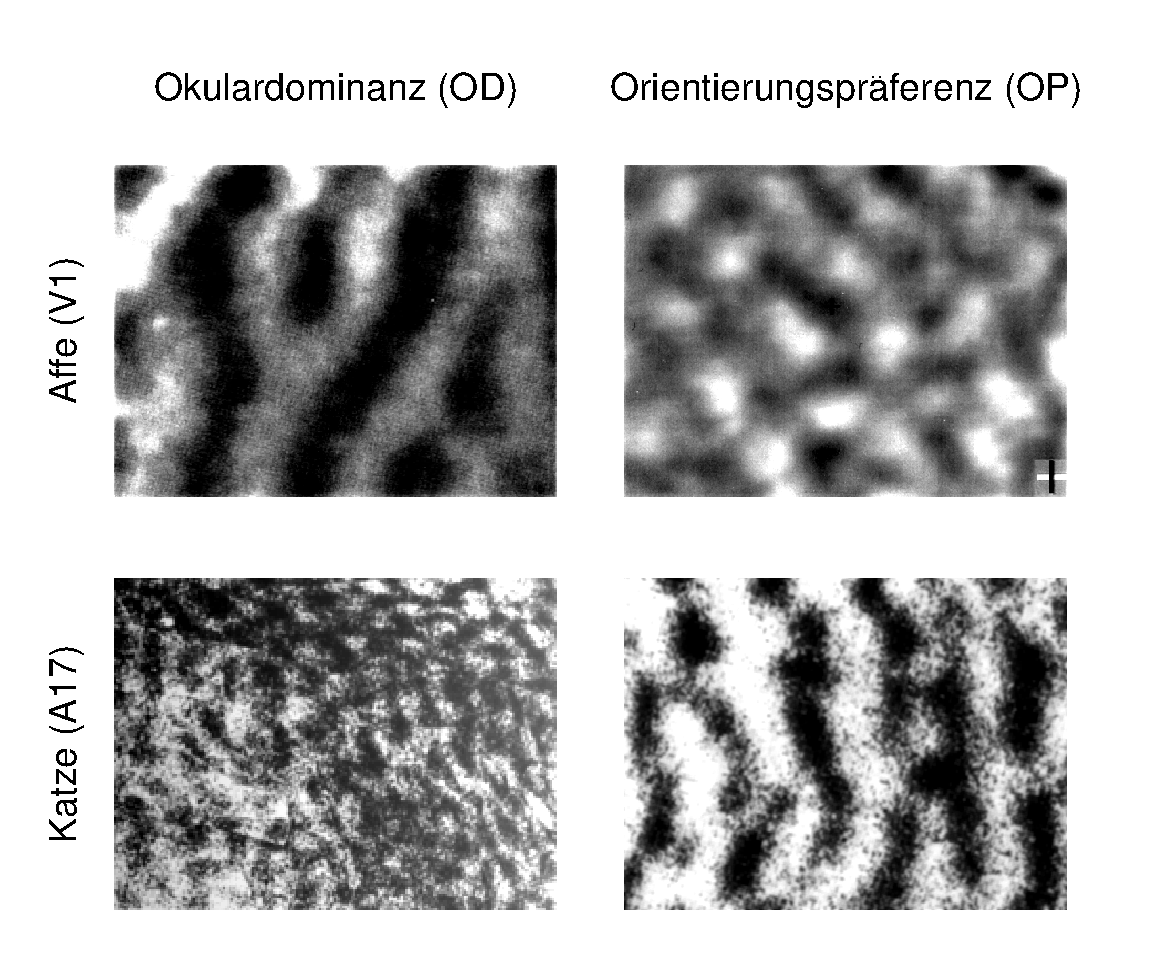
\epsfig{file=pics/monkeycat.eps,width=11cm}
\caption{Layoutvergleich kolumnärer Strukturen aus dem primären visuellen
Cortex von Katzen \protect\citeaffixed{loewel:1987,loewel:1990}{Daten aus} und Affen
\protect\citeaffixed{blasdel:1992a}{Daten aus}.}
\label{layout}

\begin{center}
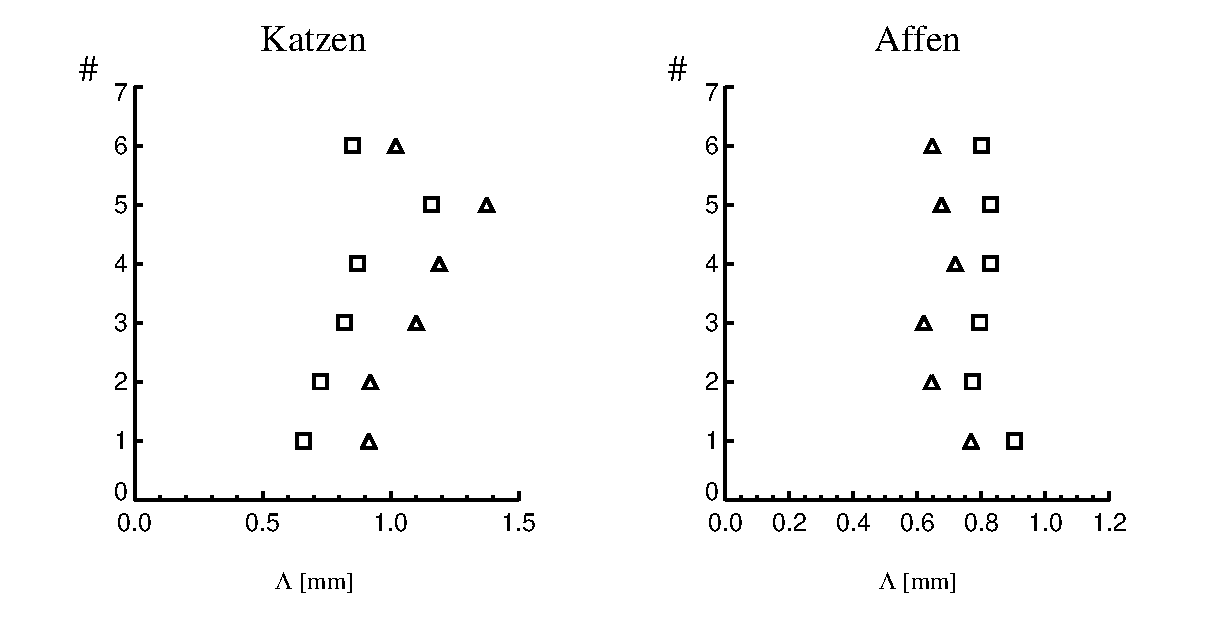
\epsfig{file=pics/wavelength.eps,width=10cm}
\end{center}
\caption{Wellenlängenvergleich typischer Orientierungspräferenz-- und
Okulardominanzkarten aus dem primären visuellen Cortex von Katzen und
Affen. Gezeigt ist das Verhältnis der Wellenlänge der
Orientierungspräferenz~($\triangle$) zur Wellenlänge der
Okuardominanz~($\square$) für mehrere Katzen
\protect\citeaffixed{loewel:1988}{links, Daten aus} und Affen
\protect\citeaffixed{oby:1993b}{rechts, Daten aus}.}
\label{wavelength}
\end{figure}

Vergleicht man nun neuronale Karten aus dem primären visuellen Cortex von
Affen und Katzen, so erkennt man, daß sich sowohl die
Orientierungspräferenz-- (OP) als auch Okulardominanzkarten (OD) in beiden
Spezies unterscheiden. Der erste, auffälligste Unterschied betrifft das
Layout der jeweiligen Karten (siehe Abb~\ref{layout}): Während eine
typische Okulardominanzkarte aus V1 des Affen ein hochreguläres Muster
paralleler Bänder aufzeigt, die senkrecht zu den Arealgrenzen verlaufen
und kaum verzweigen \cite{levayetal:1985,grinvald:1991}, besteht die
typische Okulardominanzkarte aus A17 der Katze aus einem Geflecht perliger,
aneinandergereihter Domänen ohne erkennbare Vorzugsrichtung
\cite{andersonetal:1988,loewel:1987}.  Eine ``single--condition''
Orientierungskarte dagegen, d.h. eine Karte, die für einen Stimulus einer
bestimmten, festen Orientierung erhalten wurde, besteht im Affen aus
perligen, aneinandergereihten Domänen während dieselbe Karte in der Katze
eine streifige Struktur paralleler Bänder aufzeigt.  Berücksichtigt man
nur das Layout, so erscheint eine OD--Karte aus der Katze mit einer
OP--Karte aus dem Affen vergleichbar (und eine OP--Karte aus der Katze mit
einer OD--Karte aus dem Affen siehe dazu Abb.~\ref{layout}).

Ein weiterer Unterschied der Karten in beiden Spezies betrifft die
Wellenlänge~$\Lambda$ der jeweiligen Strukturen
(vgl. Abb~\ref{wavelength}): Ein Vergleich der Wellenlänge der
OD--Struktur mit der Wellenlänge der OP--Struktur aus V1 des Affen ergibt,
daß die mittlere Wellenlänge der OD--Domänen immer größer ist als die
der OP--Domänen.  Das Verhältnis
$\Lambda_{\text{OD}}/\Lambda_{\text{OP}}$ ist ungefähr $6/5$
\cite{oby:1993b}. In der Katze verhält es sich genau umgekehrt: Hier ist
die mittlere Wellenlänge der OP--Struktur immer größer als die der
OD--Struktur; das Verhältnis $\Lambda_{\text{OD}}/\Lambda_{\text{OP}}$
beträgt ungefähr $4/5$ \cite{loewel:1988}.

Okulardominanzkarten aus dem primären visuellen Cortex von Katzen und
Affen unterscheiden sich neben ihrer charakteristischen Wellenlänge um ein
weiteres Merkmal: Der Grad der \emph{Okulardominanzsegregation} --- also
der Grad der Selektivität der Zellen für eines der beiden Augen --- ist
im Affen sowie in der strabismischen und normalsichtigen Katze
unterschiedlich stark ausgeprägt (siehe Abb.~\ref{okuhist}).

\begin{figure}[t]
\centering
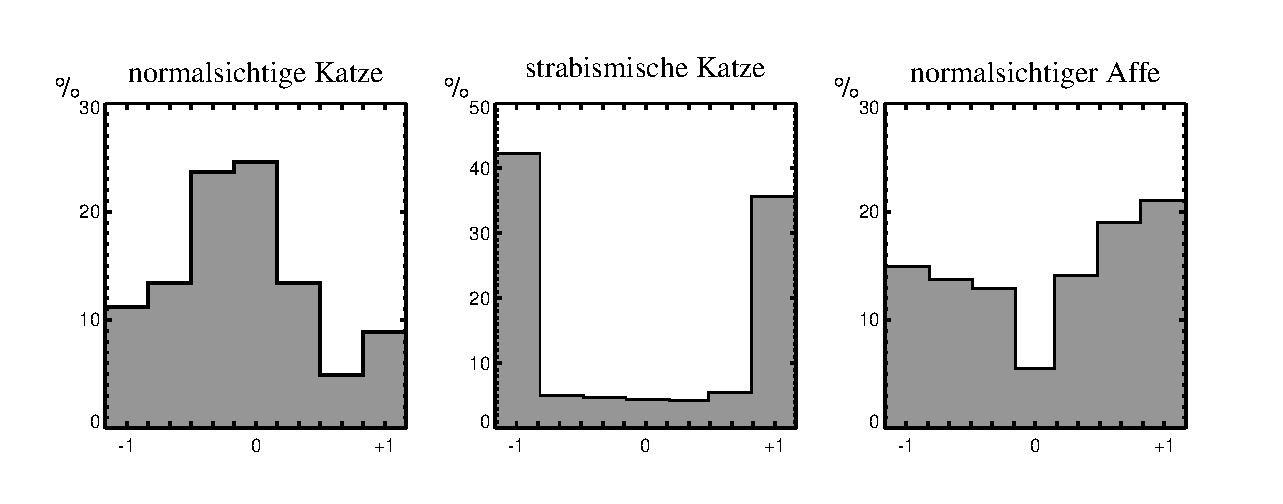
\epsfig{file=pics/okuhist.eps,width=\textwidth}
\caption{Okulardominanzhistogramme für normalsichtige und strabismische
Katzen, sowie für den Affen. Es ist die relative Häufigkeit der Zellen,
die sich entweder nur vom linken ($-1$) oder nur vom rechten ($+1$) oder
von beiden Augen ($0$) stimulieren lassen aufgetragen. Bei normalsichtigen
Katzen sind die meisten Zellen binokular. Bei strabismischen Katzen und
beim Affen überwiegt die Zahl der Zellen, die sich auf eines der beiden
Augen spezialisiert hat \protect\citeaffixed{hubel:1989}{Daten aus}.}
\label{okuhist}
\end{figure}

\subsection[Geometrische Beziehung zwischen
Iso--Orientierungslinien$\ldots$]{Geometrische Beziehung zwischen
Iso--Orientierungslinien und Oku\-lar\-do\-minanz--Grenzlinien}
\label{90grad}

Untersuchungen von Okulardominanz-- und Orientierungskarten aus V1 des
Makaken ergaben, daß es eine geometrische Beziehung zwischen den Grenzen
der Okulardominanzdomänen und den Iso--Orientierungslinien gibt
\cite{bartfield:1992,oby:1993b}: In allen untersuchten Fällen zeigt die
Statistik ihrer Schnittwinkel einen Trend zu stumpfen Winkeln (siehe
z.B. Abb~\ref{odop_hist}, rechts).

Für die Katze liegt eine solche Untersuchung bislang noch nicht vor, da in
der normalsichtigen Katze der Grad der Okulardominanzsegregation zu schwach
ist, um optisches Ableiten der Okulardominanzkarte zu erlauben (die
Signalstärke ist hier zu gering). Normalerweise wird die
Orientierungskarte in der Katze durch optisches Ableiten, eine
evtl. benötigte Okulardominanzkarte aus dem gleichen Tier jedoch mit
neurophysiologischen Methoden (vgl. Abschn.~\ref{odkarten}) gewonnen. Es
erweist sich dabei insbesondere als schwierig, die beiden auf
unterschiedliche Art und Weise gewonnenen Karten örtlich wieder zur
Deckung zu bringen. Dies wiederum ist natürlich Vorraussetzung, um eine
solche Schnittwinkelstatistik mit einem vertrauenswürdigem Maß an
Genauigkeit erstellen zu können.

\begin{figure}[t]
\centering
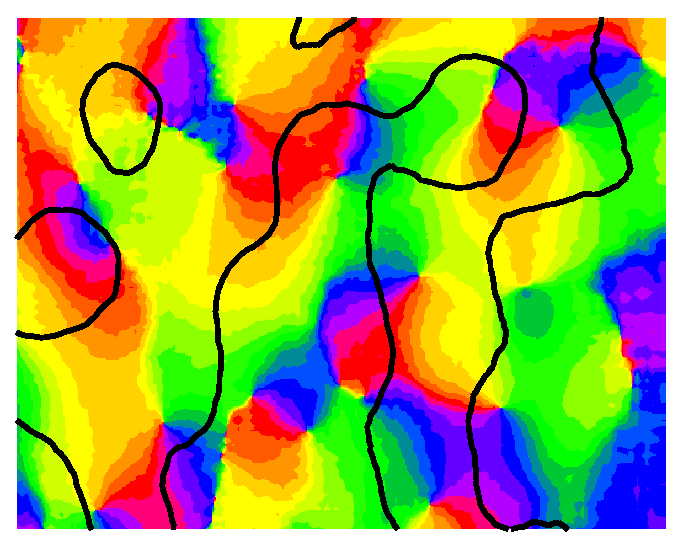
\epsfig{file=pics/odop_pict.eps,width=12.2cm}
\caption{Orientierungskarte aus A17 einer strabismischen Katze. Überlagert
dargestellt (schwarze Linien) sind die Grenzen zwischen den links-- und
rechtsäugigen Domänen der im gleichen Experiment gemessenen
Okulardominanzkarte.}
\label{odop_pict}
\end{figure}

Anhand von Okulardominanz-- und Orientierungskarten aus A17 strabismischer
Katzen, die in Experimenten von Siegrid Löwel am Max--Planck--Institut
für Hirnforschung gemessen wurden, konnte nun erstmals auch für die Katze
eine solche Schnittwinkelstatistik erstellt werden. Bei strabismischen
Katzen ist der Grad der Okulardominanzsegregation sogar stärker als im
Affen (vgl. Abschn.~\ref{unterschiede}, Abb.~\ref{okuhist}), und daher auch
die Okulardominanzkarte durch optisches Ableiten zugänglich. Diese
experimentell gemessenen Karten liegen dabei als Bildmatrix vor (die im
Experiment verwendete CCD--Kamera liefert Bilder mit einer Auflösung von
$128\times 128$ Pixeln). Eine Überlagerung eines Ausschnittes des Bildes
der Orientierungskarte $\theta(\mathbf{x})$ mit dem Bild der Grenzlinien
der Okulardominanzkarte\footnote{Für jede Position $\mathbf{x}$ liegt ein
Wert zwischen $-1$ (linkes Auge) und $+1$ (rechtes Auge) vor. Die
Grenzlinie ist somit definiert als $o(\mathbf{x}) = 0$.} $o(\mathbf{x})$
zeigt Abb.~\ref{odop_pict}. Hier wird schon durch Augenschein wird
deutlich, daß die Grenzen der Okulardominanzdomänen die
Iso--Orientierungsgebiete häufig senkrecht schneiden.
\setcounter{footnote}{1}

Um diesen Zusammenhang zu quantifizieren, benötigt man die Schnittwinkel
zwischen den Iso--Orientierungslinien $\theta(\mathbf{x})=\theta_k$ und den
Okulardominanzgrenzlinien $o(\mathbf{x}) = 0$.  Die Richtung dieser
Konturen ist in jedem Punkt über Drehung der Feldgradienten bestimmbar;
über das Skalarprodukt dieser Gradienten erhält man die Schnittwinkel
$\alpha$ für jeden Punkt $\mathbf{x}$ der Matrix:

\begin{equation*}
\alpha(\mathbf{x})=\text{acos}\!\left(\frac{\pmb\nabla\theta(\mathbf{x})
\;\pmb\nabla o(\mathbf{x})}{\vert\pmb\nabla\theta(\mathbf{x})\;\pmb\nabla
o(\mathbf{x})\vert}\right)
\end{equation*}

Zur Berechnung des räumlichen Gradienten $\pmb\nabla =
{\binom{\partial_1}{\partial_2}}$ auf dem Gitter wurde die diskrete
Approximation
\begin{equation*}
(\pmb\nabla\theta)_{ij}\approx\frac{1}{2\Delta}{\binom{\theta_{i+1,j}\,-\,\theta_{i-1,j}}{\theta_{i,j+1}\,-\,\theta_{i,j-1}}}
\end{equation*}
verwendet (analog für $\pmb\nabla o$). Das Histogramm über die
resultierende Verteilung der Schnittwinkel auf den
Okulardominanzgrenzlinien $\alpha(\left\{\mathbf{x}^\prime\vert\;
o(\mathbf{x}^\prime)=0\right\})$ für den Datensatz in Abb.~\ref{odop_pict}
zeigt Abb.~\ref{odop_hist}, Mitte. In allen vorliegenden Datensätzen aus
insgesamt 7 untersuchten strabismischen Katzen wurde eine solche
$90^\circ$--Statistik der Schnittwinkelverteilung vorgefunden
\citeaffixed{loewel:1996}{siehe}.

Ein wichtiges Phänomen visueller Reizräpresentationen sowohl bei Affen,
als auch wie hier gezeigt bei Katzen, ist demnach die lokale geometrische
Beziehung zwischen den Iso--Orientierungslinien und den Grenzen der
Okulardominanzdomänen: Diese schneiden sich mit überwiegend stumpfen
Winkeln.

\begin{figure}[t]
\centering
\epsfig{file=pics/odop_hist.eps,width=\textwidth}
\caption{Histogramme der Schnittwinkelverteilung zwischen den
Iso--Orien\-tier\-ungs\-linien und den Grenzlinien der Okulardominanzdomänen
im phänomenologischen Modell (siehe Abschn.~\ref{modell}), der
strabismischen Katze \protect\citeaffixed{loewel:1996}{hier für den in
Abb.~\ref{odop_pict} gezeigten Datensatz; weitere siehe} und den Affen
\protect\citeaffixed{oby:1993b}{Daten aus}.}
\label{odop_hist}
\end{figure}

\subsection{Entstehung neuronaler Karten durch Selbstorganisation}
\label{plastizitaet}

Die in den letzten Abschnitten skizzierte, besondere funktionale Anordnung
der Neurone im visuellen Cortex von Katzen und Affen wirft zwei
grundlegende Fragen auf \cite{marlsburg:1973}:

\begin{itemize}
\item Warum sind die Neurone so angeordnet?
\item Durch welche Mechanismen wird die Entstehung und Anordnung dieser
neuronalen Eigenschaften determiniert?
\end{itemize}

In der Diskussion um den Entstehungsmechanismus neuronaler Karten ist dabei
eine immer wiederkehrende Hypothese, daß die diesen Karten
zugrundeliegende Verschaltung der Neurone genetisch prespezifiziert sein
könnte \citeaffixed{wiesel:1974,goedecke:1996}{vgl.}. Die Kodierung der
Struktur solcher Reizrepräsentationen --- die nicht nur im visuellen
Cortex sondern auch in allen anderen Sinnessytemen angelegt sind --- im
Erbgut würde jedoch ein immenses Maß an genetischer Information
benötigen.  Ein weiteres Argument, das diese Hypothese unplausibel
erscheinen läßt, ist die Tatsache, daß mit streng genetisch
determinierten Verschaltungen nicht der im Experiment beobachtete hohe Grad
der \emph{Plastizität} visueller Reizrepräsentationen zu erklären wäre.

Eine Vielzahl von Experimenten belegt jedoch eindrucksvoll, daß die
Struktur --- zumindest aber die Feinstruktur --- visueller
Reizrepräsentationen von der visuellen Erfahrung abhängt. So führt
z.B. der Verschluß eines Auges in einem entwicklungsphysiologisch
kritischem Zeitraum nach der Geburt sowohl bei Katzen als auch bei Affen zu
einer deutlichen Abnahme des Anteils binokularer Neurone. Die meißten
Neurone antworten nach einem gewissen Zeitraum nur noch auf das geöffnete
Auge \citeaffixed{shatz:1978,levay:1980}{siehe z.B.}. Auch die Struktur der
Orientierungskarte ist reizabhängig; jedoch gibt es hierzu aufgrund der
schwierigeren Aufzucht der Tiere nicht dieselbe Fülle an Experimenten wie
für die Okulardominanz. \citeasnoun{blakemore:1970} zogen z.B. Katzen in
einer Umgebung auf, die nur aus horizontalen und vertikalen Reizen bestand:
Der Anteil der auf horizontal/vertikal spezialisierten Neurone
vergrößerte sich dadurch auf Kosten der sonstig orientierten Neurone.

Daß die Anzahl der für einen Sinnesreiz verantwortlichen Neurone mit der
Häufigkeit des Autftretens des Reizes zusammenhängt, ist dabei schon aus
anderen Sinnesbereichen bekannt.  So sind z.B. für die tastsensiblen
Fingerkuppen mehr Neurone verantwortlich als für einen vergleichbar
großen Ausschnitt des Ellenbogenbereichs. Die zahlreichen
Deprivationsexperimente am visuellen System von Katzen und Affen zeigen
deutlich, daß diese Anzahl in einem dynamischen Prozeß an eine
veränderte Reizumgebung angepaßt werden kann.

Die Basis für diese Adaptionsfähigkeit des Gehirns ist dabei nach
heutigem Kenntnistand die Variabilität der Verbindungsstärken zwischen
den Neuronen.  Die Veränderung der Verbindungsstärken findet vorwiegend
an \emph{Synapsen}, den ``Kontaktstellen'' zwischen den Neuronen statt.
Nach einer auf \citeasnoun{hebb:1949} zurückgehenden Vorstellung ändert
sich die Wirksamkeit einer Synapse in Abhängigkeit von der Korrelation
zwischen den Aktivitäten des \emph{präsynaptischen}, d.h. des die Synapse
ansteuernden, und des \emph{postsynaptischen}, d.h. des von der Synapse
angesteuerten Neurons. Diese Vorstellung konnte an einzelnen Synapsen auch
experimentell nachgewiesen werden \cite{brown:1990,kirkwood:1994}.  Die
Hebb'sche Lernregel ermöglicht die Ausrichtung der Architektur des
Nervensystems an die Struktur der Umwelt, wobei wichtige, d.h. häufig
vorkommende Ereignisse, stärker berücksichtigt werden als unwichtige
(seltene). Anhand dieser Lernregel kann das Hirn unüberwacht signifikante
Merkmale aus der Umwelt extrahieren.

Eine viel plausiblere Hypothese für die Entstehung visueller
Reizrepräsentationen ist daher, daß diese ihre Struktur spontan durch
einen Prozeß aktivitätsabhängiger Selbstorganisation ausbilden.  Zum
einen bedarf die Kodierung von Selbstorganisationsregeln im Erbgut --- die
leicht abgewandelt vielleicht auch in anderen Sinnessystemem zur Geltung
kommen könnten --- eines viel geringeren Maßes an genetischer
Information.  Viel wesentlicher ist aber, daß die aktivitätsabhängige
Selbstorganisation einen geeigneten Mechanismus zur Erklärung der
beobachteten Plastizität der Reizrepräsentationen darstellt.

    \section{Das elastische Netz}
\label{modell}
\thispagestyle{plain}

Um die Entwicklung von Orientierungs-- oder Okulardominanzkarten mittels
aktivit"atsabh"angiger Selbstorganisation zu beschreiben wurde eine
Vielzahl von Modellen vorgeschlagen.  Das Gros der Studien dient der
Untersuchung von Mechanismen, die eine Entwicklung organisierter rezeptiver
Felder aus einer realtiv undifferenzierten Anfangssituation erkl"aren
k"onnen. Hebb'sche Mechanismen allein k"onnen bereits spontane
Strukturbildung durch Symmetriebrechung bewirken \cite{linsker:1986}.  So
kann z.B. auch die Entstehung orientierungsselektiver, corticaler Zellen
durch Hebb'sche Kompetition zwischen OFF-- und ON--Eing"angen beschrieben
werden~\cite{miller:1994}.

Aus vielen Deprivationsexperimenten (siehe Abschn.~\ref{plastizitaet}) ist
bekannt, da"s die den visuellen Karten unterliegende Struktur der
geniculo--corticalen Projektion innerhalb einer kritischen Phase in einem
plastischen Zustand verbleibt.  Die Dauer dieser kritischen Phase liegt bei
mehreren Monaten \cite{hubel:1970}.  Neuere Untersuchungen zeigen, da"s
diese Periode lang im Vergleich zu der prim"aren Entstehung der Karten
ist. Sowohl in der Katze als auch im Affen ist die Orientierungskarte schon
eine Woche nach Augen"offnung etabliert
\cite{bonhoeffer:1995,blasdel:1995}.  Es ist daher plausibel, die auf
dieser Projektion basierenden Reizrepr"asentationen in adulten Tieren am
Ende der kritischen Phase als stabilen Gleichgewichtszustand fortlaufender
Auf-- und Abbauprozesse zu betrachten.

Von den bislang vorgeschlagenen Modellen sind einzig die Vertreter der
Modellklasse der sogenannten \emph{neuronalen Merkmalskarten} in der Lage,
das Ergebnis eines solchen Prozesses zu beschreiben. Die resultierende
Karte ist hier Fixpunkt einer nichtlinearen Dynamik.  Interessanterweise
sind die Modelle aus dieser Klasse bis heute auch die einzigen, die das in
Abschnitt~\ref{90grad} beschriebene, geometrische Verh"altnis zwischen
Iso--Orientierungslinien und OD--Grenzlinien korrekt reproduzieren k"onnen
\citeaffixed{erwin:1995}{vgl. Abb.~\ref{odop_hist},links und }.

Im folgenden untersuchen wir den von \citeasnoun{durbin:1991}
vorgeschlagenen Vertreter dieser Modellklasse, das sogenannte
\emph{elastische Netz}. \citeasnoun{durbin:1987} haben diesen Algorithmus,
der auf dem von \protect\citeasnoun{marlsburg:1976} vorgeschlagenen ``tea
trade model'' basiert, zuerst auf die L"osung des
NP--harten Optimierungsproblems des Handlungsreisenden angewandt.

Das elastische Netz beschreibt die Dynamik von Vektoren $\mathbf{R(x)}$ ---
die sich als rezeptive Felder interpretieren lassen --- in einem abstrakten
Reizraum $\cal S$.  Jeder dieser Vektoren geh"ort zu einem
Neuron~$\mathbf{x}$ auf einer zweidimensionalen Cortexschicht~$\cal T$.
Die neuronale Karte zu einem bestimmten Zeitpunkt~$t$ ist durch die
Konfiguration aller Merkmalsvektoren $\mathbf{R(x)}$ zu diesem Zeitpunkt
gegeben.  Die Anpassung der Merkmalsvektoren $\mathbf{R(x)}$ an die sie
aktivierenden Stimuli $\mathbf{S}$ wird durch die Gleichung

\begin{equation}
\delta\mathbf{R(x)}=\epsilon\left[\mathbf{S-R(x)}\right]
e(\mathbf{x})\;+\;\eta\Delta \mathbf{R(x)}
\label{lernschritt}
\end{equation}

beschrieben, wobei $\epsilon$ die Lernschrittweite und $e(\mathbf{x})$ die
Erregunsantwort auf die Reize $\mathbf{S}$ darstellt.  Der zweite Term der
Lernregel~\eqref{lernschritt} erzwingt dabei die Nachbarschaftserhaltung im
Zielareal~$\cal T$ ($\Delta$ ist der Laplace--Operator in zwei
Dimensionen): benachbarte Neurone tendieren dazu, "ahnliche rezeptive
Felder auszubilden. Der Parameter $\eta$ bestimmt die St"arke des
Nachbarschaftsterms.

Diese Lernregel verschiebt die rezeptiven Felder der durch $e(\mathbf{x})$
erregten Neurone in Richtung des pr"asentierten Reizes. Die rezeptiven
Felder dieser Neurone werden dadurch den sie erregenden Reizen "ahnlicher.
Die Erregungsfunktion

\begin{equation}
e(\mathbf{x|S,R})=\frac{\exp\left(-[\mathbf{S-R(x)}]^2/2\sigma^2\right)}
{\int_{\cal
T}\!d\mathbf{x}^\prime\;\exp\left(-[\mathbf{S-R(\mathbf{x}^\prime)}]^2/2
\sigma^2\right)}
\label{erregungsfunktion}
\end{equation}

\noindent bestimmt das Gebiet der Neurone in der Cortexschicht, die auf den
pr"asentierten Stimulus $\mathbf{S}$ antworten, und die Gr"o"se ihrer
Erregung.  Sie beschreibt den ``weichen Wettbewerb'' im elastischen Netz:
alle Neurone, die innerhalb des Erregungsgebietes liegen, nehmen anteilig
des Ausma"ses ihrer Erregung am Lernschritt teil.  Die Normierung
in~\eqref{erregungsfunktion} beschr"ankt die Gesamterregung in der
Cortexschicht~$\cal T$, und erzwingt die Konkurrenz der
Neurone~$\mathbf{x}$ um die Reize~$\mathbf{S}$.  Der Parameter $\sigma$
bestimmt die Gr"o"se des Gebietes im Reizraum, durch das eine einzelne
Zelle erregt wird und dadurch indirekt die Gr"o"se eines, durch einen
einzelnen Stimulus hervorgerufenen Erregungsgebietes in der simulierten
Cortexschicht.  In der N"aherung kleiner Lernschrittweiten~$\epsilon$ und
vieler Stimuli~$\mathbf{S}$ l"a"st sich die Dynamik des elastischen Netzes
durch die nichtlineare Integro--Differentialgleichung

\begin{eqnarray}
\frac{\partial}{\partial t}\, \mathbf{R(x)} &=&\int\limits_{\cal
S}\!\!d\mathbf{S}\; \rho(\mathbf{S})\; [\mathbf{S-R(x)}]\;
\frac{\exp\left(-[\mathbf{S-R(x)}]^2/2\sigma^2\right)}{\int_{\cal T} 
\!d\mathbf{x}^\prime\; \exp\left(-[\mathbf{S-R(\mathbf{x}^\prime)}]^2/2\sigma^2\right)}\;\nonumber\\
&&+\;\eta\,\Delta\mathbf{R(x)}
\label{endyn}
\end{eqnarray}

beschreiben. Diese Kontinuumsformulierung erm"oglicht einen analytischen
Zugang zu den Musterbildungsmechnismen dieses Modells
(vgl. Abschnitt~\ref{stabilitaet}).  In der Dynamik~\eqref{endyn}
bezeichnet $\rho(\mathbf{S})$ die Wahrscheinlichkeitsdichte der
Reizverteilung. Das elastische Netz minimiert die Energiefunktion

\begin{equation}
E=-\; \sigma^2\!\!\int\limits_{\cal S}\!\!d\mathbf{S}\; \rho(\mathbf{S})\;
\ln\!\!\int\limits_{\cal T}\!\!d\mathbf{x}^\prime\;
\text{e}^{-\frac{[\mathbf{S-R(\mathbf{x}^\prime)}]^2}{2\sigma^2}}+\;
\frac{\eta}{2}\!\int\limits_{\cal T}\!\!d\mathbf{x}^\prime\;
\left(\nabla\mathbf{R(\mathbf{x}^\prime)}\right)^2.
\label{energie}
\end{equation}

Sie ist, da $(\mathbf{S,R})$ auf einen endlichen Bereich des $\mathbb{R}^n$
fallen, nach unten beschr"ankt und garantiert somit die Existenz eines
Fixpunktes der Dynamik~\eqref{endyn}.  F"ur die Untersuchung der
koordinierten Entwicklung visueller Reizrepr"asentationen verwenden wir die
folgende Darstellung f"ur die RF--Parameter einer Zelle:

\begin{equation*}
\mathbf{R(x)} = \bigl[R_x(\mathbf{x}),\, R_y(\mathbf{x}),\,
r\cos(2\phi(\mathbf{x})),\, r\sin(2\phi(\mathbf{x})),\, o(\mathbf{x})\bigr]
\end{equation*}

Das Antwortverhalten einer Zelle an einem Ort $\mathbf{x}$ in der
simulierten, zweidimensionalen Cortexschicht $\cal T$ wird durch
f"unf abstrakte Merkmale beschrieben: \emph{Position} ($R_x,R_y$) des
rezeptiven Feldes im visuellen Feld, \emph{Orientierungsselektivit"at}
($r$), \emph{bevorzugte Orientierung} ($\phi$) und \emph{Okulardominanz}
($o$).  Der abstrakte Reizraum ${\cal S}$ ist folglich eine Teilmenge
des $\mathbb{R}^5$.

\subsection{Stabilit"atsanalyse}
\label{stabilitaet}

Die Dynamik des elastischen Netzes besitzt eine einfache, homogene L"osung
$\mathbf{R}_0(\mathbf{x}) = (x,\, y,\, 0,\, 0,\, 0) $. Dieser Zustand ist
gekennzeichnet durch die Abwesenheit kolumn"arer Strukturen: Alle Neurone
sind binokular und zeigen keine Orientierungsselektivit"at. Die spontane
Strukturbildung in den kolumn"aren Dimensionen wird von der Stabilit"at
dieser homogenen L"osung in Bezug auf r"aumlich periodische St"orungen
$\boldsymbol{\delta}(\mathbf{x}) = \mathbf{R(x)}-\mathbf{R}_0(\mathbf{x})$
bestimmt.  \citeasnoun{hohenstein:1994} f"uhrte eine lineare
Stabilit"atsanalyse des elastischen Netzes f"ur ${\cal
S}\subset\mathbb{R}^2$ und ${\cal T}=\mathbb{R}$ durch.  F"ur den
vorliegenden Fall ( ${\cal S}\subset\mathbb{R}^5$ und ${\cal
T}=\mathbb{R}^2$) ergibt sich f"ur die linearisierte Dynamik von
$\boldsymbol{\delta}(\mathbf{x})$

\begin{small}
\begin{eqnarray*}
\frac{\partial}{\partial t}\, \mathbf{\boldsymbol{\delta}(x)} &=&
-\int\limits_{\cal S}\!\!d\mathbf{S}\; \rho(\mathbf{S})\;
e^{-\frac{[\mathbf{S-R_0(x)}]^2}{2\sigma^2}}\;
\biggl\{\mathbf{\boldsymbol{\delta}(x)}\biggr.+\frac{1}{\sigma^2}
[\mathbf{S-R_0(x)}]\, \pmb{\Bigl<}\!\left[\mathbf{S-R_0(x)}\right]\pmb{\Big|\,
\delta}\mathbf{(x)}\pmb{\Bigr>}\nonumber\\
&&\qquad-\frac{1}{\sigma^2}\frac{[\mathbf{S-R_0(x)}]}{\text{I}\mathbf{(S)}^2}
\biggl.\int\limits_{\mathbb{R}^2}\!\!d\mathbf{x}^\prime\;
e^{-\frac{[\mathbf{S-R_0(\mathbf{x}^\prime)}]^2}{2\sigma^2}}\,
\pmb{\Bigl<}\!\left[\mathbf{S-R_0(\mathbf{x}^\prime)}\right]\pmb{\Big|\,
\delta}\mathbf{(\mathbf{x}^\prime)}\pmb{\Bigr>}\biggr\}\; +\; \ldots\nonumber\\ &&+\;
\eta\Delta\mathbf{\boldsymbol{\delta}(x)}\qquad\qquad
\label{lindyn}
\end{eqnarray*}
\end{small}

\noindent mit $\text{I}\mathbf{(S)} = 2\pi \sigma^2 \prod_{i=3}^5
\exp\left({-\frac{S_i^2}{2\sigma^2}}\right)$; $\pmb{\left<\cdot|\cdot\right>}$ bezeichnet
das Skalarprodukt in $\mathbb{R}^5$.  F"ur die kolumn"aren Dimensionen
($i=3,4,5$) erh"alt man durch L"osen der Integrale

%\begin{small}
\begin{eqnarray*}
\frac{\partial}{\partial t}\, \delta_i(\mathbf{x}) &=& -\delta_i(\mathbf{x})
+\frac{\left<S_i^2\right>}{\sigma^2}\delta_i(\mathbf{x})-\frac{\left<S_i^2 
\right>}{2\pi \sigma^2}\int\limits_{\mathbb{R}^2}\!\!d\mathbf{x}^\prime\;
e^{-\frac{\mathbf{(x-x^\prime)}^2}{4\sigma^2}}\delta_i(\mathbf{x}^\prime)\nonumber\\
&& +\; \eta\Delta\delta_i(\mathbf{x}).
\end{eqnarray*}
%\end{small}

In diese linearisierte Dynamik gehen nur noch die Varianzen
$\left<S_i^2\right>$ der Reizverteilung $\rho(\mathbf{S})$ ein.  Da die
Dynamik~\eqref{endyn} translationsinvariant ist, wird der linearisierte
Integraloperator in Fourierdarstellung diagonal.  Man erh"alt

%\begin{small}
\begin{eqnarray*}
\frac{\partial}{\partial t}\,
\Tilde{\delta}_i(\mathbf{k})&=& \lambda_i(k)\;
\Tilde{\mathbf{\delta}_i}(\mathbf{k})\\
\text{mit}\quad\lambda_i(k)&=&\left(-1+\frac{\left<S_i^2\right>}{\sigma^2}-
\frac{\left<S_i^2\right>}{\sigma^2}\; e^{-k^2\sigma^2}-\eta
k^2\right)\nonumber
\end{eqnarray*}
%\end{small}

Die Eigenwerte $\lambda_i(k)$ bestimmen die Stabilit"at der homogenen
L"osung bez"uglich einer St"orung mit Wellenzahl $k = |\mathbf{k}|$ (und
Wellenl"ange $\Lambda = 2 \pi / k$).  Alle St"orungen, bei deren Wellenzahl
$k$ der zugeh"orige Eigenwert $\lambda_i(k)$ negativ ist, zerfallen exponentiell: die homogene L"osung
bleibt stabil. Die St"orungen, zu deren Wellenzahl $k$ ein positiver
Eigenwert geh"ort, werden vertst"arkt: Es bildet sich Struktur in den
entsprechenden Dimensionen. $\lambda_i (k)$ hat genau ein Maximum bei

\begin{equation}
k_{max}=\frac{1}{\sigma} \sqrt{\ln(\left<S_i^2\right>/\eta)}
\label{kkrit}
\end{equation}

\noindent (siehe Abb.~\ref{spektrum}a). Das Maximum ist positiv f"ur alle
$\sigma <\sigma^\ast$, wobei

\begin{equation}
\sigma^\ast_i=\sqrt{\left<S_i^2\right>-\eta-\eta \ln(\left<S_i^2\right>/\eta)}.
\label{sigkrit}
\end{equation}

\begin{figure}[t]
\begin{center}
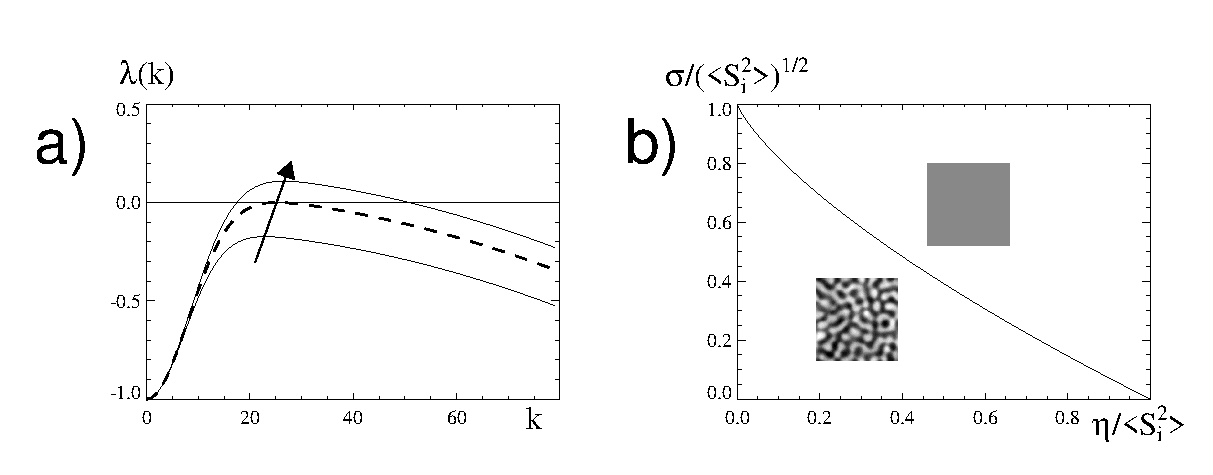
\epsfig{file=pics/analysis.eps,width=\textwidth}
\caption{\textbf{a)} Eigenwertspektrum $\lambda(k)$ 
der linearisierten Dynamik f"ur verschiedene Werte von
$\sigma$ (der Pfeil skizziert die Richtung wachsenden $\sigma$'s). Die
gestrichelte Linie zeigt das Spektrum f"ur $\sigma=\sigma^\ast$.
\textbf{b)} Phasendiagram des elastischen Netzes: Die Linie
trennt die Gebiete, in denen jeweils nur homogene bzw.  inhomogene
L"osungen stabil sind.}
\end{center}
\label{spektrum}
\end{figure}

Abbildung~\ref{spektrum}b zeigt, da"s der durch die beiden
Parameter $\sigma$ und $\eta$ aufgespannte Phasenraum des elastischen
Netzes in zwei Gebiete zerf"allt: Oberhalb der Kurve
$\sigma^\ast(\eta_{\text{rel}}),\;\text{mit}\;
\eta_{\text{rel}}=\eta/\left<S_i^2\right>$ ist die homogene L"osung,
unterhalb der Kurve  sind inhomogene L"osungen der Dynamik stabil.
H"aufig wird in Simulationen der Dynamik~\eqref{endyn} der Parameter
$\sigma$ kontinuierlich verkleinert. Da $\sigma$ in der
Potentialgleichung~\eqref{energie} als Temperatur aufgefa"st werden kann,
bezeichnet man diese Vorgehensweise  auch als ``annealing''; sie
gew"ahrleistet, da"s der resultierende Endzustand optimal auf groben und
feinen Skalen ist.

Unter der Annahme fallenden $\sigma$'s ist die Wellenzahl einer kolumn"aren
Struktur f"ur ein vorgegebenes, festes $\eta$ eine Funktion der
Stimulusvarianz $\left<S_i^2\right>$:

\begin{equation}
k_i^\ast = \sqrt{\frac{\ln\left(\left<S_i^2\right>/\eta\right)}{\left<S_i^2
\right>-\eta-\eta\ln\left(\left<S_i^2\right>/\eta\right)} }
\label{k_of_var}
\end{equation}

"Uber diese Beziehung sind die Wellenl"angen der entstehenden Strukturen an die
kritischen Kooperationsreichweiten $\sigma^\ast_i$ gekoppelt.  Die
Wellenl"angen der entstehenden kolumn"aren Strukturen sind in diesem
Fall "uber die Varianzen $\left<S_i^2\right>$ determiniert.  Die Analyse
zeigt damit, da"s die Dynamik des
elastischen Netzes   kritisch von $\sigma$ abh"angt. F"ur jede
kolumn"are Dimension existiert eine individuelle, kritische
Kooperationsreichweite $\sigma^\ast_i$, die unterschritten werden mu"s
damit sich kolumn"are Strukturen ausbilden.

\subsection{Phasen"ubergang}

\begin{figure}[t]
\begin{center}
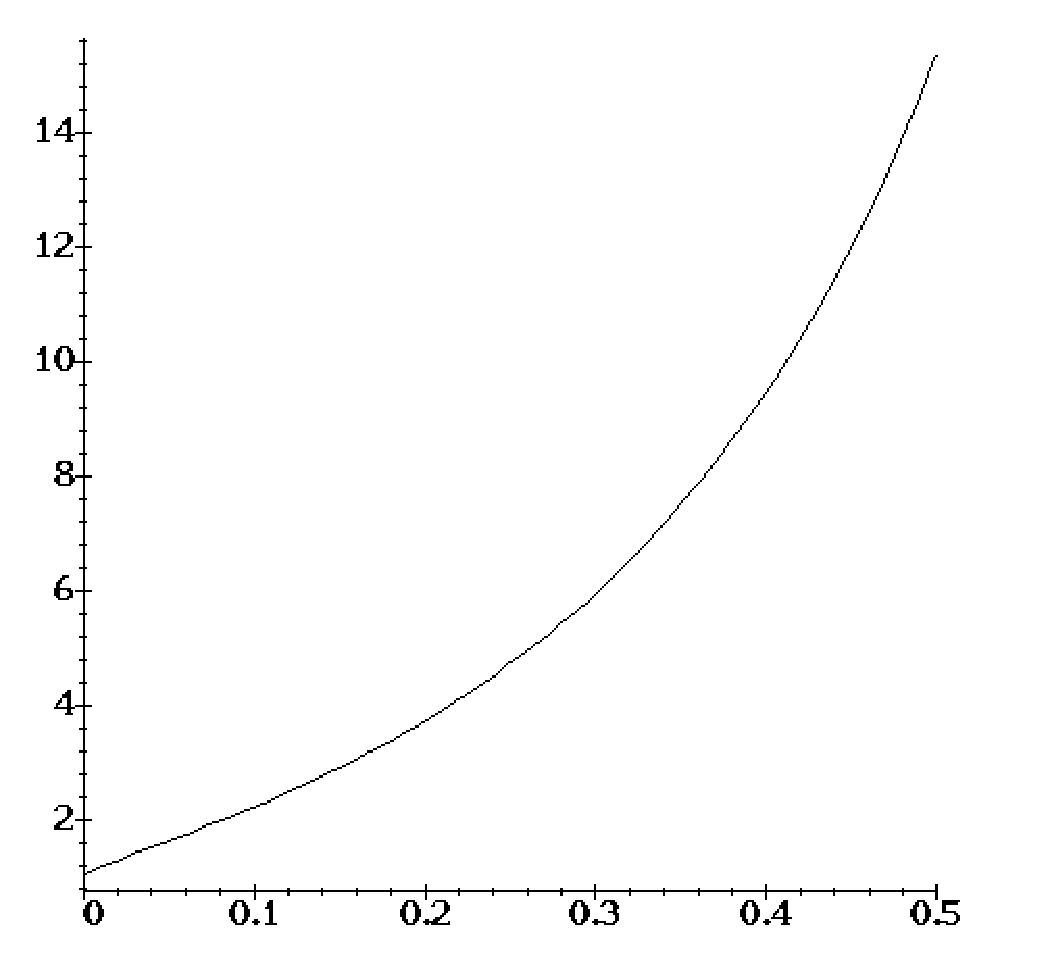
\epsfig{file=pics/koeffizient.eps,width=7cm}
\end{center}
\caption{Der Koeffizient des vierten Gliedes der Taylorentwicklung von
$E=E(A,\eta,\sigma)$ um $A$ ist eine monoton
wachsende Funktion, die bei 1 divergiert.}
\label{koeffizient}
\end{figure}

Zur Untersuchung der Frage, von welche Art der "Ubergang von homogenen zu
inhomogenen L"osungen an der Phasengrenze $\sigma^\ast(\eta_{\text{rel}})$
ist untersuchen wir die Energie f"ur die einfachste Konfiguration von $\cal
S$ und $\cal T$ mit ${\cal S} =\mathbb{R}^2$ und ${\cal T}=\mathbb{R}$. Zur
N"aherung der L"osung in N"ahe des kritischen Punktes betrachten wir den
Ansatz:

\begin{eqnarray}
\mathbf{R}_A(x)&=&{x\choose A\cos(k_{\text{max}}\,x)}
\label{ansatz}
\end{eqnarray}

Aus~\eqref{energie} ergibt sich damit die Energie $E=E(A,\eta,\sigma)$
dieser L"osung.  Die Taylorentwicklung dieser Energie um $A$ kann aus
Symmetriegr"unden nur Glieder mit geraden Potenzen enthalten.  Aus der
Entwicklung bis zur vierten Potenz ergibt sich die Amplitude der
station"aren L"osung zu

\begin{equation}
A(\sigma,\eta)=\left\{\begin{array}{cll}
0&&\sigma>\sigma^\ast\\
&&\\
\pm\sqrt{-6\,\frac{{\vrule width 0pt height 0.30cm}\partial_A^2E\big\vert_{A=0_{\phantom{g}}}}{{\vrule width 0pt height 0.4cm}\partial_A^4E\big\vert_{A=0}}}&&\sigma<\sigma^\ast
\end{array}\right.
\label{ampli}
\end{equation}

Falls der Koeffizient $\partial_A^4E\big\vert_{A=0}$ des vierten Gliedes
dieser Entwicklung positiv ist, handelt es sich um einen stetigen
"Ubergang, eine sogenannte Vorw"artsbifurkation.  Die Amplitude kann durch die
Entwicklung als Funktion der Parameter $\sigma$ und $\eta$ analytisch
angegeben werden.  In einer umfangreichen Rechnung wurden die Koeffizienten
$\partial_A^2E\big\vert_{A=0}$ und $\partial_A^4E\big\vert_{A=0}$ der
Taylorentwicklung bestimmt (die wichtigsten Schritte dazu sind in
Anhang~\ref{anhang1} aufgef"uhrt).

Es zeigt sich, da"s der Koeffizient des vierten Gliedes eine positive,
monoton wachsende Funktion ist (vgl. Abb.~\ref{koeffizient}). Der
Phasen"ubergang des elastischen Netzes ist also \emph{stetig}.  Eine
Darstellung der Gleichgewichtsamplitude $A(\eta,\sigma)$ zeigt
Abbildung~\ref{surface}. Die Amplitude steigt wie erwartet von der
kritischen Linie aus wurzelf"ormig an. F"ur kleine $\eta$ nimmt ihre
Steigung zu.

\begin{figure}[t]
\begin{center}
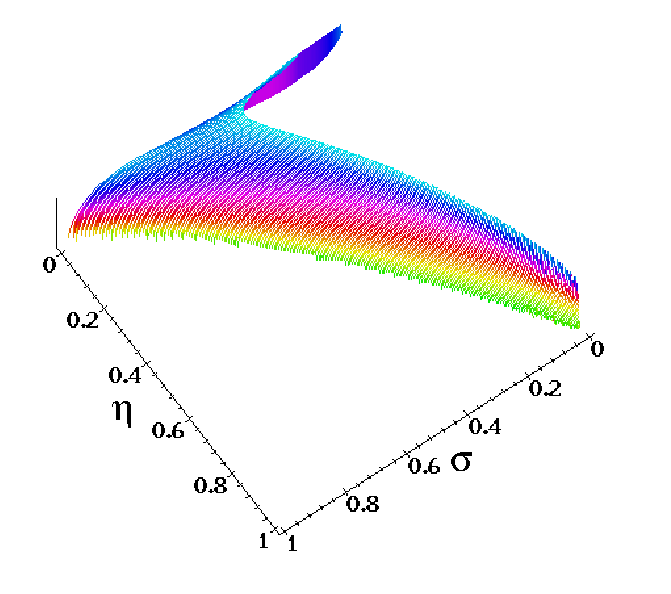
\epsfig{file=pics/surface.eps,width=10cm}
\end{center}
\caption{Amplitude~\eqref{ampli} des L"osungsansatzes~\eqref{ansatz} gezeigt
f"ur  $A\in[0\ldots0.7]$ (zur besseren "Ubersicht farbig kodiert).}
\label{surface}
\end{figure}

\subsection{Biologische Interpretation}
\label{biointerpret}

Die Analyse des elastischen Netzes in Abschnitt~\ref{stabilitaet} hat
gezeigt, da"s f"ur fest gew"ahlte Modellparameter $\sigma$ und $\eta$
kolumn"are Strukturen nur entstehen, wenn~$\sigma$ kleiner ist als ein
kritischer Wert $\sigma_i^\ast$.  Die Dynamik~\eqref{endyn} des elastischen
Netzes beschreibt ein Wechselspiel zwischen ``Konkurrenz'' und
``Kooperation''.  Jede Konfiguration der Merkmalsvektoren $\mathbf{R(x)}$
ist daher ein Kompromi"s zwischen diesen beiden ``Kr"aften'': Der
Wettbewerb der Neurone $\mathbf{x}$ um die Reize $\mathbf{S}$ treibt diese
dazu, verschiedene rezeptive Felder $\mathbf{R(x)}$ zu entwickeln. Die
Kooperation zwischen benachbarten Neuronen dagegen gleicht deren rezeptiven
Feldeigenschaften tendentiell einander an.  Die Linie im Phasendiagram
(Abb.~\ref{spektrum}b) trennt die Gebiete in denen die Kooperation
bzw. die Konkurrenz dominiert. Kooperation und Konkurrenz halten sich auf
dieser Linie die Waage. F"ur gegebenes $\sigma_i$ ist die Wellenl"ange
$\Lambda_i$ der emergierenden kolumn"aren Muster bestimmt durch

\begin{equation}
\Lambda_i = \frac{2 \pi}{\sqrt{\ln\left(\left<S_i^2\right>/\eta\right)}}\;\sigma_i
\label{lambda}
\end{equation}

Dieser Zusammenhang erlaubt es, die in biologischen Systemen nicht
me"sbaren Varianzen $\left<S_i^2\right>$ durch Vorgabe der Observablen
$\Lambda_i$ sinnvoll einzustellen.  Gleichung~\eqref{lambda} hat eine
anschauliche, biologische Bedeutung: die Wellenl"ange einer kolumn"aren
Struktur ist proportional zur typischen Gr"o"se eines, durch einen Stimulus
hervorgerufenen Erregungsgebietes. Neurone innerhalb eines solchen Gebietes
sind gleichzeitig aktiv, und haben daher die Tendenz, "ahnliche Spezifit"at
zu entwickeln. Die Erregungsgebiete wirken als ``Saatk"orner'' der
kolumn"aren Strukturen.

    \section{\mbox{Sequentielle}~\mbox{Bifurkation}~\mbox{visueller}~\mbox{Reizrepr"asentationen}}
\label{main}
\thispagestyle{plain}

Die in Abschnitt~\ref{unterschiede} vorgestellten Speziesunterschiede der
funktionalen Architektur des prim"aren visuellen Cortex laufen auf dem
ersten Blick dem Versuch einer einheitlichen Beschreibung ihrer Entstehung
zuwider.  Es ist jedoch eine plausible Annahme, da"s die Entstehung solcher
Reizrepr"asentationen in den untersuchten S"augetierarten vielleicht nicht
identischen, zumindest aber verwandten Regeln folgt
(vgl. Abschn.~\ref{plastizitaet}).  Im folgenden wird aus den in
Kapitel~\ref{modell} gewonnenen Einsichten "uber das elastische Netz ein
allgemeines Szenarium f"ur die Selbstorganisation visueller
Reizrepr"asentationen entwickelt, mit dessen Hilfe sich die in
Kapitel~\ref{biologie}, Abschnitt~\ref{unterschiede} beschriebenen
Ph"anomene einheitlich beschreiben lassen.

\subsection{Vorbetrachtungen}

Von verschiedenen Autoren wurden bereits m"ogliche Erkl"arungen dieser
Speziesunterschiede vorgeschlagen.  Es ist eine plausible Annahme, da"s die
Reichweite der lateralen Verbindungen zwischen den Neuronen einer
Zellschicht die Wellenl"ange eines kolumn"aren Musters determiniert. Diese
Vorstellung resultiert aus der "Uberlegung, da"s die Gr"o"se eines durch
einen Reiz hervorgerufenen Erregungsgebietes in einer Zellschicht mit
dieser Verbindungsreichweite verkn"upft sein sollte.  Modellsimulationen
mit unterschiedlichen lateralen Verbindungsreichweiten ergeben tats"achlich
Muster unterschiedlicher Wellenl"ange \cite{swindale:1992}.

Basierend auf dieser Annahme wurde zur Erkl"arung der verschiedenen
Wellenl"angen der OD-- und OP--Systeme vorgeschlagen, da"s sich jedes der
Systeme in einer eigenen neuronalen Schicht mit jeweils verschiedenen,
lateralen Verbindungsreichweiten zwischen den Neuronen ausbildet
\cite{loewel:1988}.  Die Autoren erwogen, da"s nicht nur die Wellenl"ange,
sondern auch die unterschiedlich ausgepr"agte ra"umliche Ordnung der Muster
(siehe Abb.~\ref{layout} und Abb.~\ref{odcorr}) mit der Gr"o"se der
lateralen Verbindungsreichweite korreliert sein k"onnte. In
Modellsimulationen der koordinierten Entwicklung von OD-- und OP--Karten
bedarf es jedoch zus"atzlicher Annahmen, um die beobachtete Anisotropie der
OD--Karte im Affen zu reproduzieren \cite{swindale:1992}.  Eine r"aumliche
Trennung der Muster verschiedener Wellenl"ange erschwert au"serdem die
Erkl"arung der lokalen geometrischen Beziehung zwischen den Mustern der
Okulardominanz und der Orientierungspr"aferenz, wie sie im visuellen Cortex
von Affen und Katzen beobachtet wird (vgl. Abschn.~\ref{90grad}).

In biologischen Systemen h"angt die Gr"o"se eines lokalen Erregungsgebietes
in einer bestimmten Zellschicht mindestens von zwei Faktoren ab: Der
Reichweite der lateralen Verbindungen der Neurone innerhalb einer
Zellschicht und der Ausdehnung der im prim"aren visuellen Cortex
terminierenden Axonen"aste.  Diese Axonen"aste stehen am Ende der
Nervenbahn (\emph{radiatio optica}, vgl. Abschn.~\ref{sehbahnkap}), die das
LGN mit dem Cortex verbindet.  Es gibt experimentelle Evidenz daf"ur, da"s
beide Gr"o"sen, sowohl die laterale Verbindungsreichweite als auch die
Ausdehnung der im Cortex terminierenden Axonen"aste, im Laufe der ersten
Lebenswochen abnehmen. Evidenz f"ur abnehmende laterale
Verbindungsreichweiten lieferten u.A. Untersuchungen am Frettchen
\cite{katz:1994}\footnote{Die Autoren dieser Arbeit diskutieren haupts"achlich
die Vergr"o"serung der langreichweitigen Verbindungen der Neurone. Jedoch
ist aus den Daten ersichtlich, da"s die lokale Verbindungsreichweite im
Laufe der Entwicklung abnimmt.}. Kleine und gro"se Axonen"aste in jungen und
adulten Katzen wurden von \citeasnoun{ferster:1978}
bzw. \citeasnoun{levay:1979} beobachtet.  Es ist also plausibel anzunehmen,
da"s die Ausdehnung eines typischen Erregungsgebietes im visuellen Cortex
im Laufe der Entwicklung abnimmt. Diese Annahme und das kritische Verhalten
des elastischen Netzes sind wichtige Vorraussetzungen f"ur das im folgenden
Abschnitt entwickelte Szenarium.
\setcounter{footnote}{1}

\subsection{Das sequentielle Bifurkationsszenarium}

\begin{figure}[t]
\begin{center}
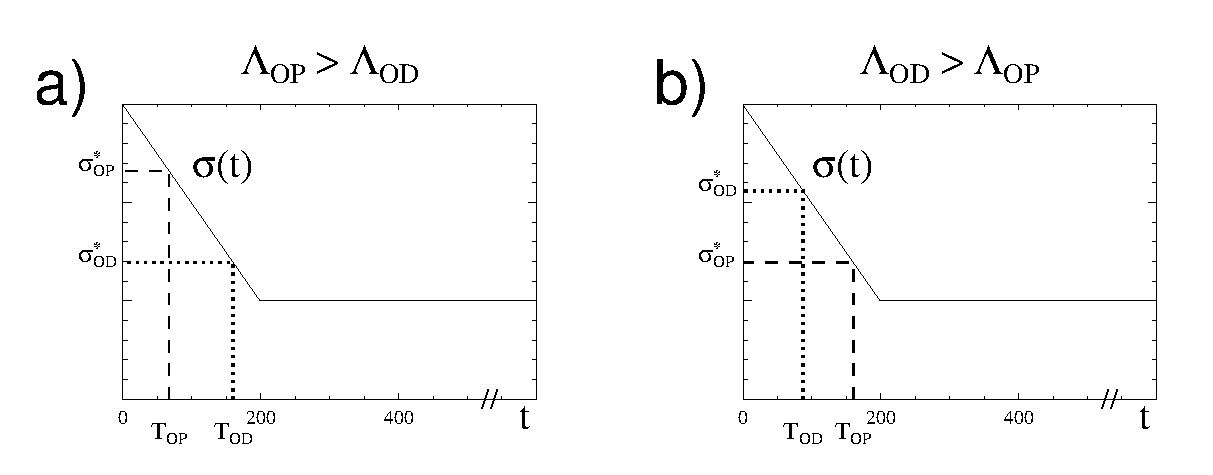
\epsfig{file=pics/seqbif.eps,width=\textwidth}
\caption{Skizze der in den Simulationen zur koordinierten Enstehung von
OD-- und OP--Mustern verwendeten Zeitentwicklung des
Modell--Parameters~$\sigma$ \textbf{a)} ``Katzen--"ahnliche'' Simulation:
Hier entsteht die Orientierungspr"aferenz zuerst, und hat daher die
gr"o"sere Wellenl"ange. \textbf{b)} ``Affen--"ahnliche'' Simulation: in
diesem Fall ensteht das Muster der Okulardominanz zuerst (und hat daher die
gr"o"sere Wellenl"ange).}
\label{zeitentwicklung}
\end{center}
\end{figure}

Wie in Kapitel~\ref{modell} dargestellt, existiert im elastischen Netz f"ur
jede emergierende kolumn"are Struktur eine unabh"angige, kritische
Kooperationsreichweite $\sigma_i^\ast$.  Diese wiederum wird durch die
Stimulusvarianz  in der entsprechenden Merkmalsraumdimension bestimmt. Die
kritischen Kooperationsreichweiten f"ur die Muster der
Orientierungspr"aferenz und die Okulardominanz werden also in der Regel
verschiedene Werte annehmen. Qualitativ sind dabei zwei F"alle zu
unterscheiden:

\begin{enumerate}
\item $\sigma_{\text{OD}}^\ast > \sigma_{\text{OP}}^\ast$ 
\item $\sigma_{\text{OD}}^\ast < \sigma_{\text{OP}}^\ast$ 
\end{enumerate}

Vor diesem Hintergrund hat die Annahme einer zeitabh"angigen, w"ahrend der
Entwicklung kontinuierlich schrumpfenden Kooperationsreichweite $\sigma(t)$
folgende Konsequenzen f"ur die Simulation der Dynamik~\eqref{endyn}: Ein
kontinuierlich abnehmendes $\sigma(t)$ unterschreitet die verschiedenen,
kritischen Kooperationsreichweiten $\sigma_i^\ast$ der 
kolumn"aren Muster \emph{sequentiell}. Zu jedem Zeitpunkt $t$, an dem
$\sigma(t)$ eine dieser kritischen Reichweiten $\sigma_i^\ast$
unterschreitet, wird die homogene L"osung in der entsprechenden Dimension
instabil; es bilden sich kolumn"are Muster mit einer durch das jeweilige
$\sigma_i^\ast$ determinierten Wellenl"ange.  Die unterschiedlichen
L"angenskalen verschiedener kolumn"arer Systeme werden also in eine
\emph{zeitliche Abfolge von Instabilit"aten} "ubersetzt. Dies bezeichnen
wir als \emph{sequentielles Bifurkationsszenarium}.  Den beiden oben
angef"uhrten Verh"altnissen von $\sigma_{\text{OD}}^{\phantom{\ast}}$ zu
$\sigma_{\text{OP}}^{\phantom{\ast}}$ entspricht damit (1.)
$\Lambda_{\text{OD}} > \Lambda_{\text{OP}}$ und (2.) $\Lambda_{\text{OD}} <
\Lambda_{\text{OP}}$.

Die in Affen und Katzen beobachteten, unterschiedlichen
Wellenl"angenverh"altnisse lassen sich mit dem sequentiellen
Bifurkationsszenarium also auf elegante Weise einheitlich erkl"aren: Das
sequentielle Bifurkationsszenarium sagt voraus, da"s sich in jeder Spezies
das Muster mit der gr"o"seren Wellenl"ange zuerst ausbildet
(vgl. Abb.~\ref{zeitentwicklung}). In Modellsimulation zum Szenarium
werden die genauen Wellenl"angenverh"altnisse notwendigerweise
reproduziert.  Inwieweit die Annahme einer unterschiedlichen
Entstehungsreihenfolge der OD-- und OP--Karten auch die r"aumliche Ordnung
dieser Karten erkl"aren kann, wird in den folgenden Abschnitten untersucht.

\subsection{Dynamische Umordnung der Okulardominanz}
\label{odord}

\begin{figure}[t]
\begin{center}
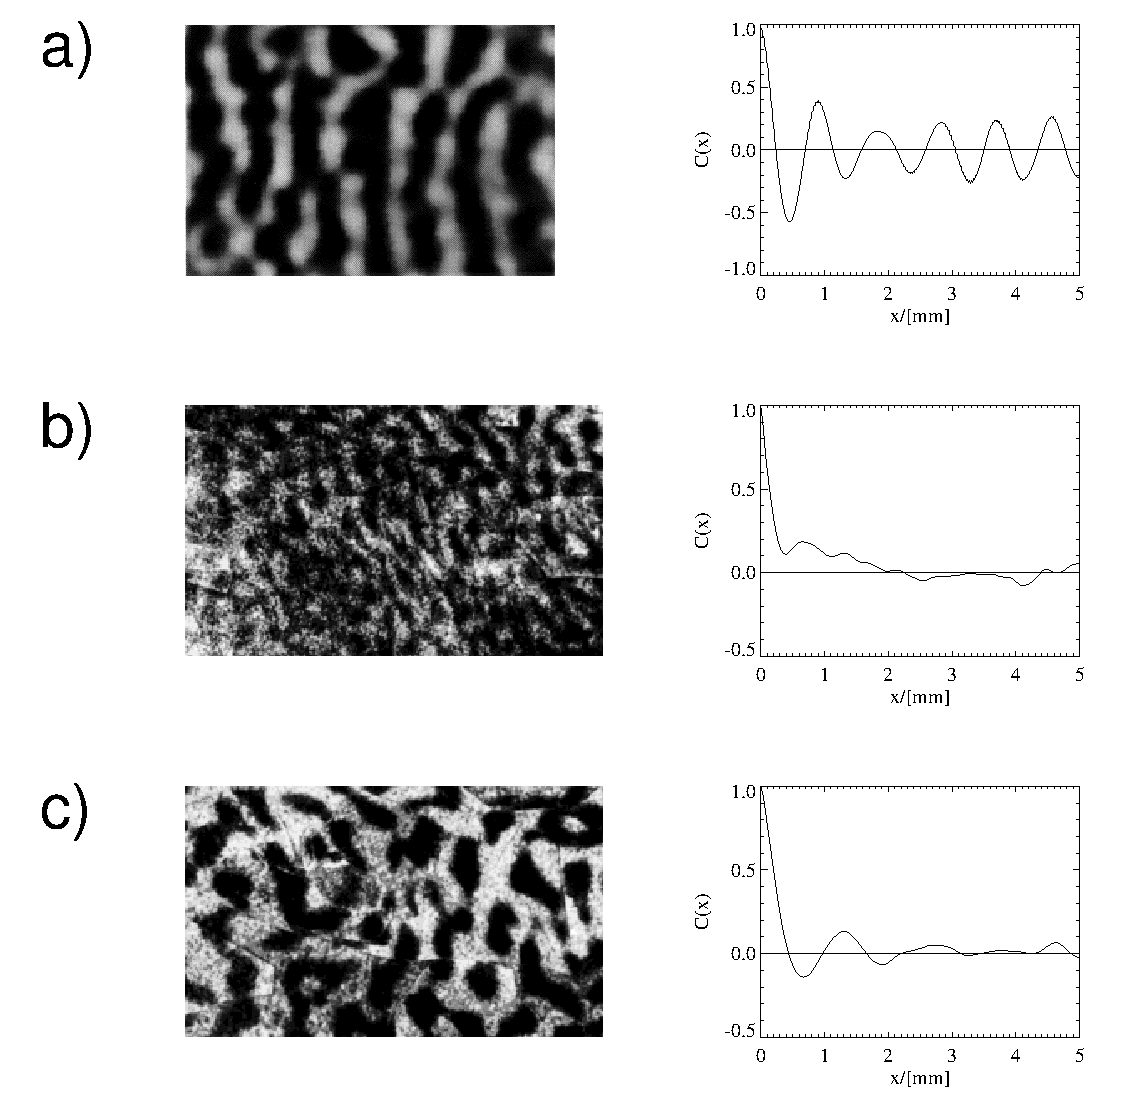
\epsfig{file=pics/od_corr.eps,width=11.9cm}
\end{center}
\caption{Die Bilder zeigen typische Auschnitte des OD--Musters aus V1 eines
Affen \protect\citeaffixed{grinvald:1991}{6.4mm$\times$4.3mm, optisches
Ableiten,} und aus A17 einer normalsichtigen und strabismischen Katze
\protect\citeaffixed{loewel:1987}{jeweils 5mm$\times$3mm, [$^3$H]--Prolin
Markierung,}. Neben jedem Bild ist die dazugeh"orige Autokorrelation
$C(\mathbf{r})\vert_{\mathbf{r}={x\choose 0}}$ gezeigt.}
\label{odcorr}
\end{figure}

\begin{figure}[t]
\begin{center}
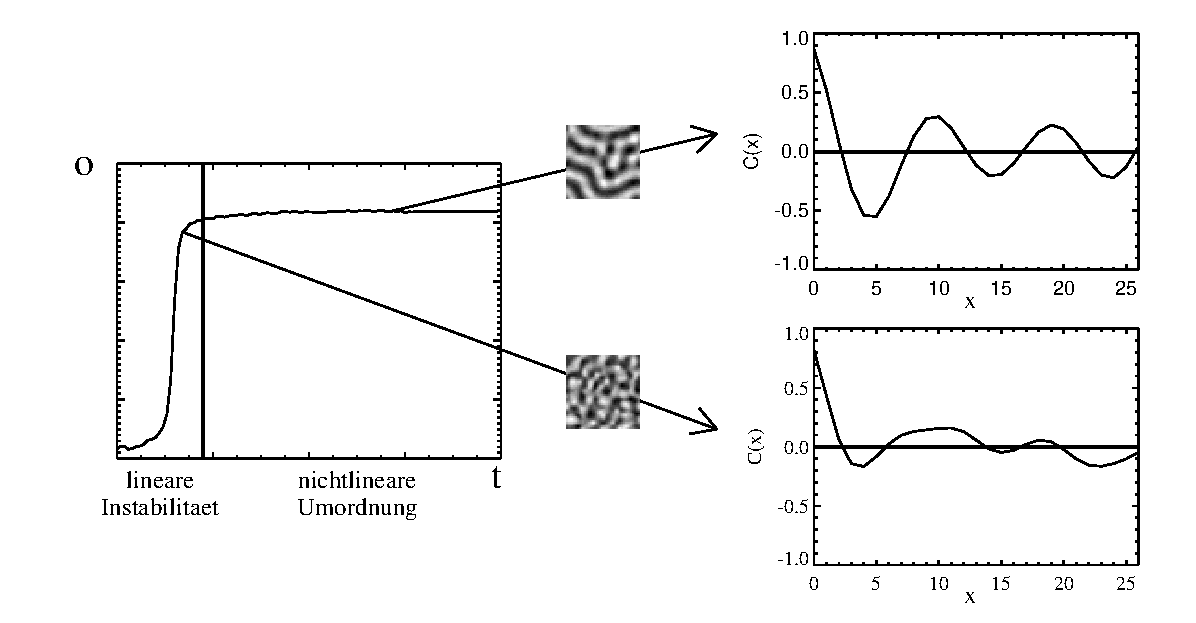
\epsfig{file=pics/umordnung.eps,width=\textwidth}
\end{center}
\caption{Simulation der Okulardominanz mit dem elastischen Netz. Links:
typische Entwicklung der Amplitude der instabilen L"osung. Rechts:
Autokorrelation eines typischen OD--Musters kurz und lange nach der
Instabilit"at.}
\label{umordnung}
\end{figure}

Das Muster der Okulardominanz im Affen zeigt einen hohen Grad r"aumlicher
Koh"arenz (vgl. Abschn.~\ref{unterschiede}): Die OD--Dom"anen bilden ein
System paralleler Streifen, die selten verzweigen und haupts"achlich
senkrecht zum Arealrand verlaufen \citeaffixed{levayetal:1985}{siehe
z.B.}. Um diese Ordnung des Musters zu quantifizieren wurde die
Autokorrelation

\begin{small}
\begin{equation}
C(\mathbf{r})=\left<\left(O(\mathbf{x+r})-\bar{O}\right)\ast\left(O(\mathbf{x})-\bar{O}\right)\right>_{\mathbf{x}\,\in\,\text{Bild}},\;\;\bar{O}=\left<O(\mathbf{x})\right>_{\mathbf{x}\,\in\,\text{Bild}}
\label{autocorr} 
\end{equation}
\end{small}

\noindent digitalisierter OD--Karten von Affen, strabismischen und
normalsichtigen Katzten berechnet.  Im gezeigten Ausschnitt aus der
OD--Karte des Affen sieht man die globale Vorzugsrichtung der Dom"anen
eutlich.  Dieser Augenschein wird durch die einige Perioden anhaltende
Modulation der Autokorrelation best"atigt (siehe Abb.~\ref{odcorr}).
Dagegen zerf"allt die Autokorrelation sowohl der OD--Karte der
strabismischen als auch der normalsichtigen Katze in allen Richtungen
schnell. Die Dom"anen dieser beiden Muster zeigen keine detektierbare
Vorzugsrichtung\footnote{Interessanterweise ist die Monokularit"at der
Zellen in A17 strabismischer Katzen st"arker ausgepr"agt als in V1 des
Affen (vgl. Abschn.~\ref{unterschiede}, Abb.~\ref{okuhist}).  Also l"a"st
sich weder der Grad der Monokularit"at der Neurone noch die Reichweite
ihrer lateralen Verbindungen zur Erkl"arung der unterschiedlichen
Anisotropie der OD--Muster in Katzen und Affen heranziehen.}.
\setcounter{footnote}{1}

Die in Simulationen aufgrund der Isotropie der Dynamik
hervorgebrachten Strukturen sind notwendigerweise statistisch isotrop
(siehe Abschn.~\ref{stabilitaet}).  Der ersten Etablierung eines solchen
Musters durch einen linearen Instabilit"atsmechanismus kann jedoch 
eine Phase der kontinuierlichen, nichtlinearen Umordnung folgen.  Simulationen der Entstehung von Okulardominanzkarten mit
dem elastischen Netz~\eqref{endyn} zeigen, da"s das Muster tats"achlich in
dieser nichtlinearen Umordnungsphase anisotrop wird und sich in ein System
paralleler Streifen umordnet (siehe Skizze in
Abb.~\ref{umordnung}).

\subsection{Ergebnisse numerischer Simulationen zum Szenarium}
\label{numerg}

Zur Erzeugung kolumn"arer Strukturen die sich durch das sequentielle
Bifurkationsszenarium ergeben wurde die Dynamik~\eqref{endyn} ausgehend vom
Anfangszustand $\mathbf{R}_0(\mathbf{x}) = (x,\, y,\, 0,\, 0,\, 0) $ f"ur
ein endliches Cortexareal $\cal T$ mit periodischen Randbedingungen
numerisch integriert (f"ur Details dazu siehe Anhang~\ref{anhang2}).

In einer Reihe von  Simulation  wurden die Stimulusvarianzen in den
Merkmalsdimensionen der Orientierungspr"aferenz und Okulardominanz  so
eingestellt, da"s nicht nur $\sigma^\ast_{\text{OP}}>\sigma^\ast_{\text{OD}}$
(und damit $\Lambda_{\text{OP}} > \Lambda_{\text{OD}}$,
vgl. Abb.~\ref{zeitentwicklung}a), sondern auch
das aus A17 der Katze bekannte Verh"altnis der Wellenl"angen beider
Muster (vgl.~Abschn.~\ref{unterschiede}, Abb.~\ref{wavelength})
erhalten wurde.  In Simulationen mit kontinuierlich schrumpfenden
$\sigma(t)$ entsteht dann das Muster der Orientierungspr"aferenz vor dem
Muster der Okulardominanz (siehe Abb.~\ref{opod}).

\begin{figure}[p]
\begin{center}
\begin{sideways}
\epsfig{file=pics/opod_rot.eps,height=\textwidth}
\end{sideways}
\end{center}
\caption{Momentaufnahmen der koordinierten Entwicklung von Okular\-do\-minanz--
und Orientierungskarten f"ur
$\sigma^\ast_{\text{OP}}>\sigma^\ast_{\text{OD}}$ (Szenarium
Abb.~\ref{zeitentwicklung}a). Die Farb--/Grauwertintensit"at spiegelt
die Amplitude der Strukturen wieder ($40\times 40$ Neurone mit periodischen
Randbedingungen, $\eta_{\text{rel}}=0.0025$,
$\sigma^\ast_{\text{OD}}=0.0837$, $\sigma^\ast_{\text{OP}}=0.1189$
$\Longrightarrow$ $\Lambda_{\text{OD}}/\Lambda_{\text{OP}}=4/5$).}
\label{opod}
\end{figure}

\begin{figure}[p]
\begin{center}
\begin{sideways}
\epsfig{file=pics/odop_rot.eps,height=\textwidth}
\end{sideways}
\end{center}
\caption{Momentaufnahmen wie oben, jedoch in einer Simulation mit
$\sigma^\ast_{\text{OD}}>\sigma^\ast_{\text{OP}}$, ensprechend des Szenariums in
Abb.~\ref{zeitentwicklung}b ($40\times 40$ Neurone mit
periodischen Randbedingungen, $\eta_{\text{rel}}= 0.0025$,
$\sigma^\ast_{\text{OD}}=0.0976$, $\sigma^\ast_{\text{OP}}=0.0679$
$\Longrightarrow$ $\Lambda_{\text{OD}}/\Lambda_{\text{OP}}=6/5$).}
\label{odop}
\end{figure}

In einer weiteren Reihe von Simulationen wurde die zweite Variante des
Szenariums (Abb.~\ref{zeitentwicklung}b) untersucht: Die Varianzen der
Reizverteilungen in den Merkmalsdimensionen wurden entsprechend des f"ur
den Affen geltenden Wellen\-l"angen\-ver\-h"altnisses gew"ahlt. Da hier
$\Lambda_{\text{OD}} > \Lambda_{\text{OP}}$ ist, entsteht in Simulationen
mit kontinuierlich schrumpfenden~$\sigma(t)$ also das Muster der
Okulardominanz vor dem Muster der Orientierungspr"aferenz (siehe
Abb.~\ref{odop}).

Abbildung~\ref{simres} stellt die Endkonfigurationen der in den
Abbildungen~\ref{opod} und \ref{odop} gezeigten, typischen
Simulationsergebnisse zu diesem Szenarium nocheinmal vergleichend vor.  Im
einen Fall (Abb.~\ref{opod} und Abb.~\ref{simres}, links) bildet die
Okulardominanz perlige Dom"anen. Die Grenzlinien dieser Dom"anen verlaufen
dabei oft geschlossen um die Singularit"aten der Orientierungskarte.  Im
anderen Fall bildet das Muster der Okulardominanz ein System ausgedehnter
Streifen, die selten verzweigen und "uber weite Abschnitte parallel
verlaufen (Abb.~\ref{odop} und Abb.~\ref{simres}, rechts).
In beiden F"allen des Szenariums stimmen die Ergebnisse aller durchgef"uhrten
Simulationen gut mit den experimentell beobachteten Karten "uberein. Das
nicht nur die Wellenl"angenverh"altnisse sondern, wie in Abb.~\ref{simres}
gezeigt, auch die unterschiedlichen Layouts der Muster korrekt reproduziert
werden, bedarf einer zus"atzlichen Erkl"arung.

\begin{figure}[t]
\begin{center}
\begin{minipage}[t]{6.2cm}
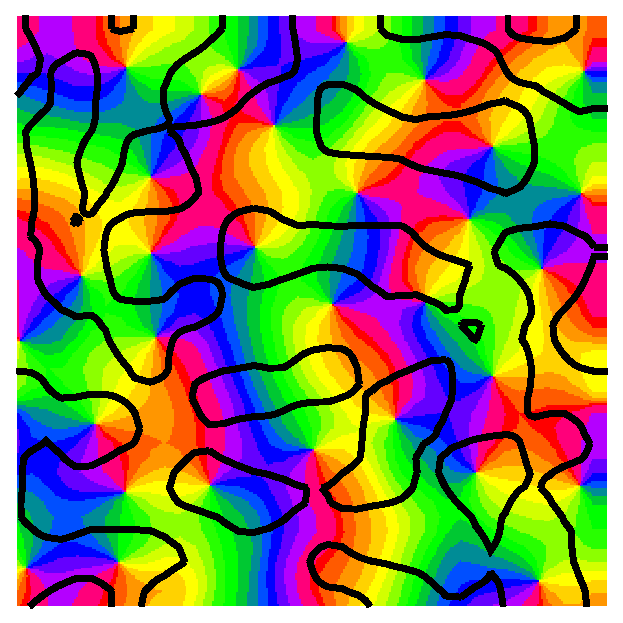
\epsfig{file=pics/op+od.eps,width=6.2cm} 
\end{minipage}
\hskip0.4cm 
\begin{minipage}[t]{6.2cm}
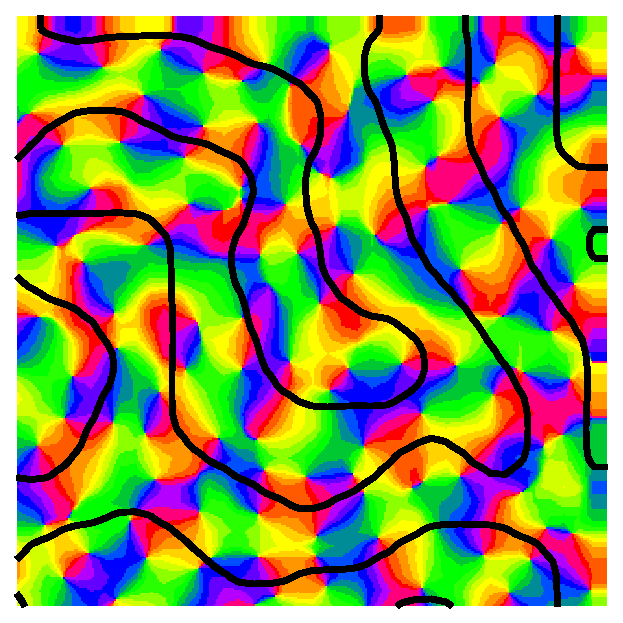
\epsfig{file=pics/od+op.eps,width=6.2cm} 
\end{minipage}
\end{center}
\caption{Vorhersage des funktionalen Layouts von Okulardominanz-- und 
Orientierungspr"aferenz--Karten f"ur die Katze (links, Ergebnis der in
Abb.~\ref{opod} gezeigten Simulation) und den Affen (rechts, Ergebnis der
in Abb.~\ref{odop} gezeigten Simulation).  Die Abbildungen zeigen eine
"Uberlagerung der Iso--Orientierungsdom"anen (farbig) mit den Grenzenlinien
der Okulardominanzkolumnen (schwarz).}
\label{simres}
\end{figure}

\begin{figure}[p]
\begin{center}
\begin{sideways}
\epsfig{file=pics/oddev.eps,height=12cm}
\end{sideways}
\end{center}
\caption{Momentaufnahmen der Weiterentwicklung einer Okulardominanzkarte.
Die am Anfang gezeigte Karte entstand in einer typischen Simulation mit
$\sigma^\ast_{\text{OP}}>\sigma^\ast_{\text{OD}}$. Ihre Weiterentwicklung in
dieser Simulation zeigt die untere Reihe. Die obere Reihe zeigt die
Weiterentwicklung der Karte \emph{ohne} das Muster der
Orientierungspr"aferenz (beide Reihen: $40\times 40$ Neurone,
$\sigma(t)=\sigma^\ast_{\text{OD}}*0.9$, $\eta_{\text{rel}}=0.001$).}
\label{oddev}
\end{figure}

\begin{figure}[p]
\begin{center}
\begin{sideways}
\epsfig{file=pics/angledev.eps,width=9cm}
\end{sideways}
\end{center}
\caption{Typische Entwicklung der geometrischen Beziehung zwischen den
Iso--Orientierungslinien und den Okulardominanz--Grenzlinien im Anschlu"s
an die prim"are Etablierung beider Strukturen.}
\label{angledev}
\end{figure}

Die Wechselwirkung der verschiedenen kolumn"aren Strukturen im elastischen
Netz f"uhrt zu einer Reproduktion der in Abschnitt~\ref{90grad}
vorgestellten, geometrischen Beziehung zwischen den
Iso--Orientierungslinien und den Grenzlinien der Okulardominanz
(vgl. \citeasnoun{erwin:1995} und Abb.~\ref{odop_hist}, links). Daher
erschient die Annahme plausibel, da"s auch im visuellen Cortex von Katzen
und Affen diese geometrische Beziehung Ergebnis einer dynamischen
Interaktion der OD-- und OP--Karten ist. In diesem Fall w"are das Muster
der Okulardominanz in der Katze ``versklavt'': Die fr"uher entstandene
Orientierungskarte w"urde die Umorganisation der Okulardominanz in ein
System parallerel B"ander mit Vorzugsrichtung verhindern.  Durch die
Wechselwirkung beider Muster im Modell bildet sich in diesem Fall die
sp"ater entstehende Okulardominanzkarte so aus, da"s ihre Grenzlinien
h"aufig geschlossene Kurven um Pinwheels bilden. Dies erf"ullt die
Randbedingung der in Abschnitt~\ref{90grad} vorgestellten, geometrischen
Beziehung beider Strukturen. 

Um diese Hypothese der Versklavung der Okulardominanz zu testen, wurde nach
der Entstehung beider Muster in Simulationen mit
$\sigma^\ast_{\text{OP}}>\sigma^\ast_{\text{OD}}$ untersucht, wie sich die
Okulardominanzkarte \emph{mit} bzw. in Abwesenheit der Orientierungskarte
weiterentwickelt. Wie Abbildung~\ref{oddev} an einem Beispiel zeigt, ordnet
sich der identische Ausgangszustand der Okulardominanzkarte ohne
Orientierungskarte in ein System paralleler B"ander mit Vorzugsrichtung um.
Unter Br"ucksichtigung der Randbedingung stumpfer Schnittwinkel zwischen
Iso--Orientierungslinien und Okulardominanz--Grenzlinien l"a"st sich also
in der Katze das Layout der Muster durch ihre sequentielle Enstehung
erkl"aren.  Ein wie im Affen beobachtetes, r"aumlich koh"arentes Muster der
Okulardominanz dagegen kann ebenfalls nur durch dynamische Umordnung in
Abwesenheit des Musters der Orientierungspr"aferenz entstehen
(vgl. Abschn.~\ref{odord}).  Aus unseren Simulationen folgt also, da"s die
Wechselwirkung der Strukturen ihr Erscheinungsbild entscheidend
beeinflu"st.

Berechnet man, wie in Abschnitt~\ref{90grad} dargelegt, die Verteilung der
Schnittwinkel zwischen den Iso--Orientierungslinien und den Grenzlinien der
Okulardominanz f"ur mehrere Konfigurationen im Zuge der Entwicklung, so
zeigt sich, das diese geometrische Beziehung beider Muster im Modell erst
in einem Zeitraum nach der prim"aren Etablierung der Muster realisiert
wird (ein Beispiel daf"ur zeigt Abb.~\ref{angledev}).  Dies wird in allen
durchgef"uhrten Simulationen der koordinierten Entwicklung von OD-- und
OP--Karten ungeachtet ihrer Entstehungsreihenfolge beobachtet und zeigt,
da"s diese geometrische Beziehung beider Muster Resultat eines dynamischen
Umordnungsprozess in der nichtlinearen Phase der Entwicklung ist.

    \section{Zusammenfassung und Diskussion}
\label{zusammenfassung}
\thispagestyle{plain}

In der vorliegenden Arbeit wurde ein Szenarium für die koordinierte
Entwicklung von Okulardominanz-- und Orientierungskarten entwickelt.  Wie
in Kapitel~\ref{main} gezeigt, bietet die aus der Sicht der Nichtlinearen
Dynamik plausible Annahme dynamischer Umordnung und Interaktion der
Okulardominanz-- und Orientierungspräferenzkarten eine einfache und
einheitliche Erklärung für die unterschiedliche Erscheinung dieser
Strukturen im visuellen Cortex von Affen und Katzen.  Das streifige
Erscheinungsbild der OD--Karte aus V1 des Affen kann durch dynamische
Umordnung des Musters nach seiner Entstehung, in Abwesenheit
orientierungsspeziefischer Zellen erklärt werden.  Die perlige Struktur
der OD--Karte in A17 der Katze wird durch die Wechselwirkung des Musters
der Okulardominanz mit der bereits etablierten Orientierungskarte
erklärt. Diese führt dazu, daß die Grenzlinien der entstehenden
OD--Domänen häufig geschlossene Kurven um Pinwheels bilden und verhindert
die Umordnung der OD--Karte in ein anisotropes Muster mit globaler
Vorzugsrichtung.

\begin{quote}
In diesem Bild wird das Layout einer neuronalen Karte also
entscheidend durch den \emph{Zeitpunkt} ihrer Entstehung bestimmt.  Dieser
spezielle Zeitpunkt bestimmt auch die Wellenlänge des Musters: Die
Vorhersage des sequentiellen Bifurkationsszenariums ist, daß in allen Spezies
die Karte mit der \emph{größeren} Wellenlänge \emph{früher} entsteht.
\end{quote}

In V1 des Affen sind nach der Geburt sowohl orientierungsselektive als auch
okulardominante Zellen vorhanden~\cite{blakemore:1978}, daher ist keine sichere
Aussage über die zeitliche Abfolge ihrer Spezialisierung möglich.
\citeasnoun{rakic:1981} beschreibt allerdings, daß die
Okulardominanzsegregation ca.~3~Wochen vor der Geburt einsetzt. Aus
A17 der Katze ist bekannt, daß hier die Zellen in einem frühen
Stadium der Entwicklung bereits orientierungsselektiv sind
\citeaffixed{movshon:1981,fregnac:1984}{siehe}, während
die Okulardominanzkarte erst im Laufe der 3.--7. Woche nach der Geburt entsteht
\cite{shatz:1978,levay:1979}. Dies stimmt mit der Vorhersage des
sequentiellen Bifurkationsszenariums überein.

\citeasnoun{jones:1991} haben eine alternative Erklärung des
unterschiedlichen Erscheinungsbildes von Okulardominanzkarten in Katzen und
Affen vorgeschlagen. Die Autoren argumentieren, daß der hohe Grad
räumlicher Kohärenz der OD--Karte im Affen Anisotropien der retinotopen
Abbildung vom Gesichtsfeld in den Cortex reflektiert. Das isotrope OD--Muster
in der Katze ist demnach Ausdruck einer isotropen retino--corticalen
Abbildung.  Die Autoren benutzen ein nicht weiter biologisch motiviertes
Optimierungsverfahren zur numerischen Evaluation ihrer
Hypothese,\footnote{\citeasnoun{bauer95b} konnte jedoch zeigen, daß sich
neuronale Merkmalskarten unter diesen Annahmen ähnlich Verhalten.} und
behandeln die Okulardominanzstruktur unabhängig von anderen, im visuellen
Cortex vorhandenen Reizrepräsentationen.  Die in Abschn.~\ref{90grad}
vorgestellte Wechselwirkung zwischen den Mustern der Okulardominanz und der
Orientierungspräferenz läßt die isolierte Untersuchung der
Okulardominanz jedoch fragwürdig erscheinen.
\setcounter{footnote}{1}

Es ist wichtig anzumerken, daß die in Kapitel~\ref{main} vorgestellten
Simulationsergebnisse keineswegs von der speziellen Wahl der
Dynamik~\eqref{endyn} abhängen, vielmehr jedoch von den folgenden,
allgemeinen Eigenschaften:

\begin{itemize}
\item die Größe eines typischen, durch einen Stimulus hervorgerufenen
Erregungsgebietes im Cortex bestimmt die Wellenlänge der entstehenden
kolumnären Struktur
\item diese Größe nimmt mit der Zeit ab
\item kolumnäre Strukturen entstehen nur unterhalb einer kritischen
Größe des Erregungsgebietes. Oberhalb dieser kritischen
Kooperationsreichweite bleibt die homogene Lösung stabil.
\end{itemize}

Jedes Modell, das diese allgemeinen Eigenschaften mit der
Dynamik~\eqref{endyn} gemeinsam hat, ist geeignet die Entstehung
kolumnärer Muster unterschiedlicher Wellenlänge anhand des sequentiellen
Bifurkationsszenariums zu beschreiben. Das hier verwendete
elastische Netz ist also nur ein Vertreter aus einer viel umfangreicheren
Klasse von Modellen. Die Verwendung des elastischen Netzes rechtfertigt
sich dabei vor allem durch den leichten analytischen Zugang zu den
Musterbildungsmechanismen dieses Modells, sowie durch den vertretbaren,
numerischen Aufwand bei der Implementierung der Dynamik auf Computern.

Die konsequente Interpretation der aktivitätsabhängigen
Selbstorganisation neuronaler Karten als dynamischer Prozess dient auch der
einheitlichen Erklärung eines anderen Speziesunterschieds.
Orientierungskarten aus V1 des Affen und A17 strabismischer und
normalsichtiger Katzen unterscheiden sich in der der Dichte ihrer
Punktdefekte: Wird zum Speziesvergleich die Dichte der Pinwheels $\rho
[1/mm^2]$ einer Orientierungskarte mit der charakteristischen Wellenlänge
$\Lambda_{\text{OP}}$ dieser Karte skaliert, so ergibt sich im Affen ein
Wert von $\hat{\rho}=\rho \Lambda_{\text{OP}}^2\approx 3.75$ ($\hat{\rho}$
mißt dann die relative Häufigkeit der Pinwheels in einem Kästchen der
Seitenlänge $\Lambda_{\text{OP}}$). In der Katze ist diese Größe immer
merklich kleiner als $3$, nach vorliegenden, z.T. unveröffentlichten
Messungen beträgt der Wert $\hat{\rho}\approx 2.4$ für normalsichtige und
$\hat{\rho}\approx 3.0$ für strabismische Katzen.

\citeasnoun{wolf:1996} konnten zeigen, daß die skalierte Dichte in allen
Spezies anfänglich größer als $\pi$ sein muß. In Tieren, in denen der
adulte Wert von $\hat{\rho}$ deutlich unter $\pi$ liegt muß dieser
geringere Wert folglich durch Annihilation von Pinwheels entgegengesetzter
Chiralität in Folge eines Umordnungsprozesses der Karte während der
Entwicklung erreicht worden sein. Das Auftreten unterschiedlicher
skalierter Pinwheeldichten $\hat{\rho}$ in verschiedenen Spezies kann unter
Berücksichtigung der Wechselwirkung zwischen den Mustern der
Okulardominanz und der Orientierungspräferenz durch die beobachtete
Korrelation der Pinwheeldichte mit dem Grad der Okulardominanzsegregation
erklärt werden.

Im Folgenden versuchen wir die Frage zu beantworten warum die kritische
Kooperationsreichweite der Okulardominanz im Affen, wie im sequentiellen
Bifurkationsszenarium gefordert, größer sein sollte als die der
Orientierungspräferenz (und aus welchen Gründen dieses Verhältnis in der
Katze dann umgekehrt ist).

Die Tendenz der Neurone, sich auf Reize aus einem Auge zu spezialisieren
wird in biologischen Systemen durch die unvollständige Korrelation der
Aktivität in den beiden Augen bestimmt: Es ist daher anzunehmen, daß
diese Tendenz der Neurone mit abnehmender Korrelation zwischen beiden Augen
zunimmt.  Dies wird auch durch Beobachtungen an strabismischen Katzen
belegt: Durch Induzierung eines künstlichen Schielwinkels sind die
Aktivitäten beider Augen völlig dekorreliert und führen zur
vollständigen Segregation der Afferenzen aus beiden Augen
(vgl. Abb.~\ref{okuhist}, Mitte).

Der kritische Wert der Kooperationsreichweite $\sigma^\ast_{\text{OD}}$ ist
im Modell ein Maß für die Tendenz der Neurone, sich auf Signale aus einem
der beiden Augen zu spezialisieren. Je größer $\sigma^\ast_{\text{OD}}$,
desto größer muß die Kooperationsreichweite der Neurone sein um die
Segregation zu verhindern. Es ist daher anzunehmen, daß dieser kritische
Wert von den Korrelationen beider Augen bestimmt wird: Wachsende
Korrelationen sollten zu einer Verkleinerung des kritischen Wertes führen.
Dies ist in der Tat in detaillierten Modellen der Okulardominanzsegregation
der Fall \cite{scherf:1994}.

Im Affen beginnt die Okulardominanzsegregation bereits vor der Geburt
\cite{rakic:1981} und erfolgt daher unter dem Einfluß
notwendigerweise dekorrelierter Spontanaktivität der beiden Retinae.  In
Katzen hingegen vollzieht sich die Entwicklung des visuellen Cortex erst
nach der Geburt, und erfolgt weitgehend unter dem Einfluß korrelierter
Aktivität aus beiden Augen nach Augenöffnung.  Mit diesem Zusammenhang
kann auch die in strabismischen Katzen beobachtete Vergrößerung der
Okulardominanzwellenlänge gegenüber normalsichtigen Katzen erklärt
werden: Der erhöhte Wert von $\sigma^\ast_{\text{OD}}$ führt analog zum
sequentiellen Bifurkationsszenarium zur früheren Entstehung des Musters,
und damit zu einer Vergrößerung der Wellenlänge
\citeaffixed{scherf:1994}{siehe auch}.

Diese Erklärung legt eine interessante Verifikation des hier entwickelten
Szenariums nahe: Sollte es durch frühste Dekorrelation der Eingangsaktivität
der Augen möglich sein, die Okulardominanzsegregation zu induzieren, bevor
sich das Muster der Orientierungspräferenzen ausbildet, so müßte sich in
diesen Katzen ein ``affenähnliches'' OD--Muster ausbilden.  Chronisches
optisches Ableiten neuronaler Karten während des Entwicklungszeitraumes
wird in zukünftigen Experimenten am visuellen Cortex einzelner Katzen oder
Affen eine geeignete Möglichkeit bieten, die in dieser Arbeit
vorgeschlagenen Mechanismen auf ihre Gültigkeit hin zu überprüfen.

\nocite{hoffsuemmer95a,hoffsuemmer96}


    \appendix
    \section{Entwicklung der Energie des elastischen Netzes}
\label{anhang1}
\thispagestyle{plain}

\noindent Wir betrachten das Potential~\eqref{energie}

\begin{small}
\begin{eqnarray}
E\left(\mathbf{R}_A(x)\right)&=&-\;\sigma^2\lim_{L\to\infty}\int\limits_{-L}^{L}\!\!\frac{1}{2L}\int\limits_{-r}^{r}\!\!\frac{1}{2r}\;\;\ln\!\!\int\limits_{-\infty}^{\infty}\!\!\!\exp\!\left(-[\mathbf{S}-\mathbf{R}_A(x)]^2/2\sigma^2\right)dx\;\;dS_y dS_x\nonumber\\
&&+\;\frac{\eta}{2}\;\lim_{L\to\infty}\int\limits_{-L}^{L}\!\!\frac{1}{2L}\;\left[\partial_x\mathbf{R}_A(x)\right]^2\;dx
\label{energieanh}
\end{eqnarray}
\end{small}

\noindent mit dem Ansatz

\begin{small}
\begin{eqnarray*}
\mathbf{R}_A(x)&=&{\binom{x}{A\cos(kx)}}.
\end{eqnarray*}
\end{small}

\noindent Die Taylorentwicklung des Potentials bis zu Gliedern der 4.~Ordnung lautet
unter diesem Ansatz:

\begin{small}
\begin{equation*}
E = E\big\vert_{A=0} \;\;+\;\;
\frac{1}{2}\partial_A^2E\big\vert_{A=0}A^2 \;\;+\;\;
\frac{1}{24}\partial_A^4E\big\vert_{A=0}A^4 \;\;+\;\; O(A^6)
\end{equation*}
\end{small}

\noindent Unter der Berücksichtigung von

\small
$$\frac{\eta}{2}\;\lim_{L\to\infty}\int\limits_{-L}^{L}\!\!\frac{1}{2L}\;\left[\partial_x\mathbf{R}_A(x)\right]^2\;dx = \frac{\eta}{2}\left(1+\frac{(Ak)^2}{2}\right)$$
\normalsize

\noindent und mit der Definition

\begin{small}
\begin{equation}
\Theta :=\int\limits_{-\infty}^{\infty}\!\!\!\exp\!\left(-[\mathbf{S}-\mathbf{R}_A(x)]^2/2\sigma^2\right)\;dx
\label{theta}
\end{equation}
\end{small}

\noindent folgt für die Energie~\eqref{energieanh} und ihre ersten vier Ableitungen:

\begin{small}
\begin{eqnarray*}
E &=& -\sigma^2 \int\!\!\!\int \ln \Theta\;\;+\;\;\frac{\eta}{2}\left(1+\frac{(kA)^2}{2}\right)\\
&&\\
\partial_A E &=& -\sigma^2 \int\!\!\!\int \frac{1}{\Theta}\,\, \partial_A\Theta\;\;+\;\;\frac{1}{2}\eta k^2A\\
&&\\
\partial_A^2 E &=& \sigma^2 \int\!\!\!\int \frac{1}{\Theta^2}\,\,\left(\partial_A\Theta\right)^2\;\;-\;\;\sigma^2\int\!\!\!\int\frac{1}{\Theta}\,\,\partial_A^2\Theta\;\;+\;\;\frac{1}{2}\eta k^2\\
\end{eqnarray*}
\end{small}

\begin{small}
\begin{eqnarray*}
\partial_A^3 E &=& -2\sigma^2\int\!\!\!\int\frac{1}{\Theta^3}\,\,\left(\partial_A\Theta\right)^3\;\;+\;\;3\sigma^2\int\!\!\!\int\frac{1}{\Theta^2}\,\,\partial_A\Theta\,\,\partial_A^2\Theta\;\;-\;\;\sigma^2\int\!\!\!\int\frac{1}{\Theta}\,\,\partial_A^3\Theta\\
&&\\
\partial_A^4 E &=&6\sigma^2\int\!\!\!\int\frac{1}{\Theta^4}\,\,\left(\partial_A\Theta\right)^4\;\;-\;\;12\sigma^2\int\!\!\!\int\frac{1}{\Theta^3}\,\,\left(\partial_A\Theta\right)^2\,\,\partial_A^2\Theta\\
&&+\;\;3\sigma^2\int\!\!\!\int\frac{1}{\Theta^2}\,\,\left(\partial_A^2\Theta\right)^2\;\;+\;\;4\sigma^2\int\!\!\!\int\frac{1}{\Theta^2}\,\,\partial_A\Theta\,\,\partial_A^3\Theta\;\;-\;\;\sigma^2\int\!\!\!\int\frac{1}{\Theta}\,\,\partial_A^4\Theta
\end{eqnarray*}
\end{small}

\noindent Die hier erscheinenden Ableitungen von $\Theta$ ergeben sich
aus~\eqref{theta} zu

\begin{small}
\begin{eqnarray*}
{\partial_A} \Theta &=&\int\limits_{-\infty}^{\infty}\!\!\!dx\; \frac{1}{\sigma^2} \cos(kx)\left[S_y-A\cos(kx)\right] \;\exp\!\left(-[\mathbf{S}-\mathbf{R}_A(x)]^2/2\sigma^2\right)\\
&&\\
{\partial^2_A}  \Theta &=& -\int\limits_{-\infty}^{\infty}\!\!\!dx\; \frac{1}{\sigma^2} \cos^2(kx) \;\exp\!\left(-[\mathbf{S}-\mathbf{R}_A(x)]^2/2\sigma^2\right) \\
&&+ \int\limits_{-\infty}^{\infty}\!\!\!dx\; \frac{1}{\sigma^4} \cos^2(kx)\left[S_y-A\cos(kx)\right]^2  \;\exp\!\left(-[\mathbf{S}-\mathbf{R}_A(x)]^2/2\sigma^2\right)\\
&&\\
{\partial^3_A}  \Theta &=& -3 \int\limits_{-\infty}^{\infty}\!\!\!dx\; \frac{1}{\sigma^4} \cos^3(kx) \left[S_y-A\cos(kx)\right] \;\exp\!\left(-[\mathbf{S}-\mathbf{R}_A(x)]^2/2\sigma^2\right) \\
&&+ \int\limits_{-\infty}^{\infty}\!\!\!dx\; \frac{1}{\sigma^6} \cos^3(kx) \left[S_y-A\cos(kx)\right]^3 \;\exp\!\left(-[\mathbf{S}-\mathbf{R}_A(x)]^2/2\sigma^2\right)\\
&&\\
{\partial^4_A}  \Theta &=& 3 \int\limits_{-\infty}^{\infty}\!\!\!dx\; \frac{1}{\sigma^4} \cos^4(kx) \;\exp\!\left(-[\mathbf{S}-\mathbf{R}_A(x)]^2/2\sigma^2\right) \\
&&- 6 \int\limits_{-\infty}^{\infty}\!\!\!dx\; \frac{1}{\sigma^6} \cos^4(kx) \left[S_y-A\cos(kx)\right]^2 \;\exp\!\left(-[\mathbf{S}-\mathbf{R}_A(x)]^2/2\sigma^2\right) \\
&&+\int\limits_{-\infty}^{\infty}\!\!\!dx\; \frac{1}{\sigma^8} \cos^4(kx) \left[S_y-A\cos(kx)\right]^4 \;\exp\!\left(-[\mathbf{S}-\mathbf{R}_A(x)]^2/2\sigma^2\right)
\end{eqnarray*}
\end{small}

\noindent Zu ihrer Berechnung benötigt man die Integrale

\begin{small}
\begin{eqnarray*}
{\cal C}1 &:=&\;\;\int\limits_{-\infty}^{\infty}\!\!dx\;\cos(kx)\;\exp\!\left(-(x-S_x)^2/2\sigma^2)\right)=\sqrt{2\pi}\sigma\;\cos(kS_x)\;{\rm e}^{(-k^2\sigma^2/2)}\\
{\cal C}2 &:=&\int\limits_{-\infty}^{\infty}\!\!dx\;\cos^2(kx)\;\exp\!\left(-(x-S_x)^2/2\sigma^2)\right)=\frac{1}{2}\sqrt{2\pi}\sigma\;\left[\cos(2kS_x)\;{\rm e}^{(-2k^2\sigma^2)}+1\right]
\end{eqnarray*}
\end{small}

\begin{small}
\begin{eqnarray*}
{\cal C}3 &:=&\int\limits_{-\infty}^{\infty}\!\!dx\;\cos^3(kx)\;\exp\!\left(-(x-S_x)^2/2\sigma^2)\right)\\
&=&\frac{1}{4}\sqrt{2\pi}\sigma\;\left[\cos(3kS_x)\;{\rm e}^{(-9k^2\sigma^2/2)}+3\cos(kS_x)\;{\rm e}^{(-k^2\sigma^2/2)}\right]\phantom{\int\limits_{-\infty}^{\infty}}\\
{\cal C} 4 &:=&\int\limits_{-\infty}^{\infty}\!\!dx\;\cos^4(kx)\;\exp\!\left(-(x-S_x)^2/2\sigma^2)\right)\\
&=&\frac{1}{8}\sqrt{2\pi}\sigma\;\left[\cos(4kS_x)\;{\rm e}^{(-8k^2\sigma^2)}+4\cos(2kS_x)\;{\rm e}^{(-2k^2\sigma^2)}+3\right]\phantom{\int\limits_{-\infty}^{\infty}}
\end{eqnarray*}
\end{small}

\noindent Daraus folgt für die Ableitungen von $\Theta$ and der Stelle $A=0$:

\begin{small}
\begin{eqnarray*}
\Theta\big\vert_{A=0} &=& \sqrt{2\pi}\sigma\;\;{\rm e}^{(-S_y^2/2\sigma^2)}\\
&&\\
{\partial_A}
\Theta\big\vert_{A=0}&=&\left(\frac{1}{\sigma^2}S_y\right)\;\;{\rm e}^{(-S_y^2/2\sigma^2)}\;\;{\big\{}{\cal C}1{\big\}}\\
&&\\
{\partial^2_A}
\Theta\big\vert_{A=0}&=&\left(-\frac{1}{\sigma^2}+\frac{1}{\sigma^4}S_y^2\right)\;\;{\rm e}^{(-S_y^2/2\sigma^2)}\;\;{\big\{}{\cal C}2{\big\}}\\
&&\\
{\partial^3_A}
\Theta\big\vert_{A=0}&=&\left(-\frac{3}{\sigma^4}S_y+\frac{1}{\sigma^6}S_y^3\right)\;\;{\rm e}^{(-S_y^2/2\sigma^2)}\;\;{\big\{}{\cal C}3{\big\}}\\
&&\\
{\partial^4_A}
\Theta\big\vert_{A=0}&=&\left(\frac{3}{\sigma^4}-\frac{6}{\sigma^6}S_y^2+\frac{1}{\sigma^8}S_y^4\right)\;\;{\rm e}^{(-S_y^2/2\sigma^2)}\;\;{\big\{}{\cal C}4{\big\}}\\
\end{eqnarray*}
\end{small}

\noindent Damit ergibt sich für die Koeffizienten der Taylorentwicklung:

\begin{small}
\begin{eqnarray*}
E\big\vert_{A=0}&=&\frac{1}{2}\;\left(-\sigma^2\ln\!\left(2\pi\sigma^2\right)+\frac{r^2}{3}+\eta\right)\\
&&\\
\partial_A E\big\vert_{A=0}&=&0\\
&&\\
\partial_A^2 E\big\vert_{A=0}&=&\frac{1}{2}\left(1-\frac{r^2}{3\sigma^2}+\frac{r^2}{3\sigma^2}\;{\rm e}^{(-k^2\sigma^2)}+\eta k^2\right)\\
&&\\
\partial_A^3 E\big\vert_{A=0}&=&0\\
&&\\
\partial_A^4 E\big\vert_{A=0}&=&\frac{1}{40\sigma^6}\;\bigg(\,\left[ 3\;{\rm e}^{(-4k^2\sigma^2)}-12\;{\rm e}^{(-3k^2\sigma^2)}+18\;{\rm e}^{(-2k^2\sigma^2)}-12\;{\rm e}^{(-k^2\sigma^2)}+3 \right] r^4\\
&&\qquad\;\;\,-\left[ 10\;{\rm e}^{(-4k^2\sigma^2)}-20\;{\rm e}^{(-3k^2\sigma^2)}+20\;{\rm e}^{(-k^2\sigma^2)}-10 \right] \sigma^2 r^2\\
&&\qquad\;\;\,+\left[ 15\;{\rm e}^{(-4k^2\sigma^2)}-15 \right] \sigma^4 \bigg)
\end{eqnarray*}
\end{small}

    \section{Numerische Integration der Dynamik}
\label{anhang2}
\thispagestyle{plain}

In allen Simulationen zum Szenarium wurde die Dynamik~\eqref{endyn}
ausgehend vom Anfangszustand $\mathbf{R}_0(\mathbf{x}) = (x,\, y,\, 0,\,
0,\, 0) $ auf einem diskreten Gitter aus $40\times 40$ bzw. $64\times 64$
Neuronen mit periodischen Randbedingungen integriert. Die Varianzen
$\left<S_i^2\right>$ der Reizverteilungen wurden dabei so gewählt, daß
die enstehenden Muster vorgegebene Wellenlängen aufweisen
(vgl. Abschn.~\ref{numerg}). Dazu wurde die Gleichung

\begin{equation*}
    \Lambda_i = \frac{2 \pi}{\sqrt{\ln\left(\left<S_i^2\right>/\eta\right)}}\;\sigma_i
\end{equation*}

\noindent numerisch invertiert. Die Gültigkeit dieser Gleichung
erfordert, daß $\sigma$ während der Simulation monoton fällt und zu
Beginn größer als das größte kritische~$\sigma^\ast$ ist. Der
Zeitverlauf von $\sigma(t)$ wurde in der Regel als linearer Abfall von den
Werten $\sigma_{\mbox{\tiny Start}}=1.1*\sigma_i^\ast$ und
$\sigma_{\mbox{\tiny Ende}}=0.9*\sigma_j^\ast$, mit
$\sigma_i>\sigma_j$ angesetzt (vgl. Abb.~\ref{zeitentwicklung}).

Die numerische Integration der Dynamik~\eqref{endyn} erfolgte dann in einem
expliziten Einschritt--Verfahren. Für den Integralterm der Dynamik wurde
ein Adams--Bashford Schritt verwendet, der diffusionsartige Anteil der
Dynamik anschließend in Fourierdarstellung exakt integriert. Dieses
Verfahren gewährleistet die numerische Stabilität des linearen Terms.
Der Integralterm wurde als Mittelwert über eine Menge von
Pseudo--Zufallsstimuli genähert. Die Anzahl der Stimuli wurde dabei so
gewählt, daß in jedes Volumenelement der linearen Ausdehnung $2\sigma$
mindestens 50 Reize fallen. Typischerweise erforderte dies ca.~20000
Stimuli pro Integrationsschritt.

Die Wahl des Integrationszeitschrittes $dt$ orientierte sich unter
Zuhilfenahme der Analytik an drei Kriterien: $dt$ sollte klein auf der
Zeitskala der linearen Instabilität, und nicht zu groß für den
Integralterm sein (dieser zeigt eine numerische Instabilität bei großen
$dt$). Außerdem sollte $dt$ klein sein gegenüber der Zerfallszeit des
Musters unter der Einwirkung des Laplace--Schritts. Diese Randbedingungen
der Wahl von $dt$ wurden durch

\begin{equation*}
    dt = \text{MIN}\left(\frac{\tau_{\mbox{\tiny
        Inst}}}{5},\frac{\tau_{\scriptscriptstyle \Delta}}{20}\right)
\end{equation*}

\noindent erfüllt, wobei $\tau_{\mbox{\tiny
    Inst}}=\frac{1}{\lambda(k_{\text{max}})}$ und $\tau_{\scriptscriptstyle
    \Delta}=\eta*k_{\text{max}}^2$. Die Zeitentwicklung einer durch die
Instabilität entstehenden Struktur wurde in einem Zeitraum von bis zu
$200\tau$ verfolgt. Eine typische Simulation nahm auf modernsten
Workstations mehrere Wochen in Anspruch.

    \clearpage
    \printbibliography
\end{document}
